% Created by tikzDevice version 0.11 on 2018-05-22 19:12:25
% !TEX encoding = UTF-8 Unicode
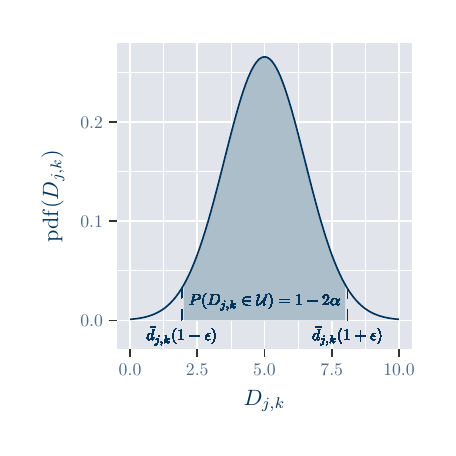
\begin{tikzpicture}[x=1pt,y=1pt]
\definecolor{fillColor}{RGB}{255,255,255}
\path[use as bounding box,fill=fillColor,fill opacity=0.00] (0,0) rectangle (144.54,144.54);
\begin{scope}
\path[clip] (  0.00,  0.00) rectangle (144.54,144.54);
\definecolor{drawColor}{RGB}{255,255,255}
\definecolor{fillColor}{RGB}{255,255,255}

\path[draw=drawColor,line width= 0.6pt,line join=round,line cap=round,fill=fillColor] (  0.00,  0.00) rectangle (144.54,144.54);
\end{scope}
\begin{scope}
\path[clip] ( 32.13, 28.37) rectangle (139.04,139.04);
\definecolor{fillColor}{RGB}{225,229,235}

\path[fill=fillColor] ( 32.13, 28.37) rectangle (139.04,139.04);
\definecolor{drawColor}{RGB}{255,255,255}

\path[draw=drawColor,line width= 0.3pt,line join=round] ( 32.13, 56.67) --
	(139.04, 56.67);

\path[draw=drawColor,line width= 0.3pt,line join=round] ( 32.13, 92.48) --
	(139.04, 92.48);

\path[draw=drawColor,line width= 0.3pt,line join=round] ( 32.13,128.29) --
	(139.04,128.29);

\path[draw=drawColor,line width= 0.3pt,line join=round] ( 49.14, 28.37) --
	( 49.14,139.04);

\path[draw=drawColor,line width= 0.3pt,line join=round] ( 73.44, 28.37) --
	( 73.44,139.04);

\path[draw=drawColor,line width= 0.3pt,line join=round] ( 97.74, 28.37) --
	( 97.74,139.04);

\path[draw=drawColor,line width= 0.3pt,line join=round] (122.03, 28.37) --
	(122.03,139.04);

\path[draw=drawColor,line width= 0.6pt,line join=round] ( 32.13, 38.77) --
	(139.04, 38.77);

\path[draw=drawColor,line width= 0.6pt,line join=round] ( 32.13, 74.58) --
	(139.04, 74.58);

\path[draw=drawColor,line width= 0.6pt,line join=round] ( 32.13,110.39) --
	(139.04,110.39);

\path[draw=drawColor,line width= 0.6pt,line join=round] ( 36.99, 28.37) --
	( 36.99,139.04);

\path[draw=drawColor,line width= 0.6pt,line join=round] ( 61.29, 28.37) --
	( 61.29,139.04);

\path[draw=drawColor,line width= 0.6pt,line join=round] ( 85.59, 28.37) --
	( 85.59,139.04);

\path[draw=drawColor,line width= 0.6pt,line join=round] (109.88, 28.37) --
	(109.88,139.04);

\path[draw=drawColor,line width= 0.6pt,line join=round] (134.18, 28.37) --
	(134.18,139.04);
\definecolor{fillColor}{RGB}{173,190,203}

\path[fill=fillColor] ( 56.43, 51.66) --
	( 57.40, 53.46) --
	( 58.38, 55.45) --
	( 59.35, 57.62) --
	( 60.32, 59.97) --
	( 61.29, 62.52) --
	( 62.26, 65.25) --
	( 63.23, 68.16) --
	( 64.21, 71.26) --
	( 65.18, 74.51) --
	( 66.15, 77.92) --
	( 67.12, 81.47) --
	( 68.09, 85.13) --
	( 69.07, 88.88) --
	( 70.04, 92.69) --
	( 71.01, 96.54) --
	( 71.98,100.38) --
	( 72.95,104.19) --
	( 73.93,107.93) --
	( 74.90,111.55) --
	( 75.87,115.03) --
	( 76.84,118.32) --
	( 77.81,121.38) --
	( 78.78,124.18) --
	( 79.76,126.69) --
	( 80.73,128.86) --
	( 81.70,130.68) --
	( 82.67,132.12) --
	( 83.64,133.17) --
	( 84.62,133.80) --
	( 85.59,134.01) --
	( 86.56,133.80) --
	( 87.53,133.17) --
	( 88.50,132.12) --
	( 89.47,130.68) --
	( 90.45,128.86) --
	( 91.42,126.69) --
	( 92.39,124.18) --
	( 93.36,121.38) --
	( 94.33,118.32) --
	( 95.31,115.03) --
	( 96.28,111.55) --
	( 97.25,107.93) --
	( 98.22,104.19) --
	( 99.19,100.38) --
	(100.17, 96.54) --
	(101.14, 92.69) --
	(102.11, 88.88) --
	(103.08, 85.13) --
	(104.05, 81.47) --
	(105.02, 77.92) --
	(106.00, 74.51) --
	(106.97, 71.26) --
	(107.94, 68.16) --
	(108.91, 65.25) --
	(109.88, 62.52) --
	(110.86, 59.97) --
	(111.83, 57.62) --
	(112.80, 55.45) --
	(113.77, 53.46) --
	(114.74, 51.66) --
	(114.74, 38.77) --
	(113.77, 38.77) --
	(112.80, 38.77) --
	(111.83, 38.77) --
	(110.86, 38.77) --
	(109.88, 38.77) --
	(108.91, 38.77) --
	(107.94, 38.77) --
	(106.97, 38.77) --
	(106.00, 38.77) --
	(105.02, 38.77) --
	(104.05, 38.77) --
	(103.08, 38.77) --
	(102.11, 38.77) --
	(101.14, 38.77) --
	(100.17, 38.77) --
	( 99.19, 38.77) --
	( 98.22, 38.77) --
	( 97.25, 38.77) --
	( 96.28, 38.77) --
	( 95.31, 38.77) --
	( 94.33, 38.77) --
	( 93.36, 38.77) --
	( 92.39, 38.77) --
	( 91.42, 38.77) --
	( 90.45, 38.77) --
	( 89.47, 38.77) --
	( 88.50, 38.77) --
	( 87.53, 38.77) --
	( 86.56, 38.77) --
	( 85.59, 38.77) --
	( 84.62, 38.77) --
	( 83.64, 38.77) --
	( 82.67, 38.77) --
	( 81.70, 38.77) --
	( 80.73, 38.77) --
	( 79.76, 38.77) --
	( 78.78, 38.77) --
	( 77.81, 38.77) --
	( 76.84, 38.77) --
	( 75.87, 38.77) --
	( 74.90, 38.77) --
	( 73.93, 38.77) --
	( 72.95, 38.77) --
	( 71.98, 38.77) --
	( 71.01, 38.77) --
	( 70.04, 38.77) --
	( 69.07, 38.77) --
	( 68.09, 38.77) --
	( 67.12, 38.77) --
	( 66.15, 38.77) --
	( 65.18, 38.77) --
	( 64.21, 38.77) --
	( 63.23, 38.77) --
	( 62.26, 38.77) --
	( 61.29, 38.77) --
	( 60.32, 38.77) --
	( 59.35, 38.77) --
	( 58.38, 38.77) --
	( 57.40, 38.77) --
	( 56.43, 38.77) --
	cycle;
\definecolor{drawColor}{RGB}{0,52,92}

\path[draw=drawColor,line width= 0.6pt,line join=round] ( 36.99, 39.14) --
	( 37.97, 39.23) --
	( 38.94, 39.34) --
	( 39.91, 39.47) --
	( 40.88, 39.63) --
	( 41.85, 39.83) --
	( 42.83, 40.06) --
	( 43.80, 40.33) --
	( 44.77, 40.66) --
	( 45.74, 41.04) --
	( 46.71, 41.49) --
	( 47.68, 42.01) --
	( 48.66, 42.62) --
	( 49.63, 43.31) --
	( 50.60, 44.12) --
	( 51.57, 45.03) --
	( 52.54, 46.07) --
	( 53.52, 47.24) --
	( 54.49, 48.55) --
	( 55.46, 50.02) --
	( 56.43, 51.66) --
	( 57.40, 53.46) --
	( 58.38, 55.45) --
	( 59.35, 57.62) --
	( 60.32, 59.97) --
	( 61.29, 62.52) --
	( 62.26, 65.25) --
	( 63.23, 68.16) --
	( 64.21, 71.26) --
	( 65.18, 74.51) --
	( 66.15, 77.92) --
	( 67.12, 81.47) --
	( 68.09, 85.13) --
	( 69.07, 88.88) --
	( 70.04, 92.69) --
	( 71.01, 96.54) --
	( 71.98,100.38) --
	( 72.95,104.19) --
	( 73.93,107.93) --
	( 74.90,111.55) --
	( 75.87,115.03) --
	( 76.84,118.32) --
	( 77.81,121.38) --
	( 78.78,124.18) --
	( 79.76,126.69) --
	( 80.73,128.86) --
	( 81.70,130.68) --
	( 82.67,132.12) --
	( 83.64,133.17) --
	( 84.62,133.80) --
	( 85.59,134.01) --
	( 86.56,133.80) --
	( 87.53,133.17) --
	( 88.50,132.12) --
	( 89.47,130.68) --
	( 90.45,128.86) --
	( 91.42,126.69) --
	( 92.39,124.18) --
	( 93.36,121.38) --
	( 94.33,118.32) --
	( 95.31,115.03) --
	( 96.28,111.55) --
	( 97.25,107.93) --
	( 98.22,104.19) --
	( 99.19,100.38) --
	(100.17, 96.54) --
	(101.14, 92.69) --
	(102.11, 88.88) --
	(103.08, 85.13) --
	(104.05, 81.47) --
	(105.02, 77.92) --
	(106.00, 74.51) --
	(106.97, 71.26) --
	(107.94, 68.16) --
	(108.91, 65.25) --
	(109.88, 62.52) --
	(110.86, 59.97) --
	(111.83, 57.62) --
	(112.80, 55.45) --
	(113.77, 53.46) --
	(114.74, 51.66) --
	(115.72, 50.02) --
	(116.69, 48.55) --
	(117.66, 47.24) --
	(118.63, 46.07) --
	(119.60, 45.03) --
	(120.57, 44.12) --
	(121.55, 43.31) --
	(122.52, 42.62) --
	(123.49, 42.01) --
	(124.46, 41.49) --
	(125.43, 41.04) --
	(126.41, 40.66) --
	(127.38, 40.33) --
	(128.35, 40.06) --
	(129.32, 39.83) --
	(130.29, 39.63) --
	(131.27, 39.47) --
	(132.24, 39.34) --
	(133.21, 39.23) --
	(134.18, 39.14);

\path[draw=drawColor,line width= 0.6pt,dash pattern=on 4pt off 4pt ,line join=round] ( 55.65, 38.77) -- ( 55.65, 50.33);

\path[draw=drawColor,line width= 0.6pt,dash pattern=on 4pt off 4pt ,line join=round] ( 55.65, 38.77) -- ( 55.65, 50.33);

\path[draw=drawColor,line width= 0.6pt,dash pattern=on 4pt off 4pt ,line join=round] ( 55.65, 38.77) -- ( 55.65, 50.33);

\path[draw=drawColor,line width= 0.6pt,dash pattern=on 4pt off 4pt ,line join=round] ( 55.65, 38.77) -- ( 55.65, 50.33);

\path[draw=drawColor,line width= 0.6pt,dash pattern=on 4pt off 4pt ,line join=round] ( 55.65, 38.77) -- ( 55.65, 50.33);

\path[draw=drawColor,line width= 0.6pt,dash pattern=on 4pt off 4pt ,line join=round] ( 55.65, 38.77) -- ( 55.65, 50.33);

\path[draw=drawColor,line width= 0.6pt,dash pattern=on 4pt off 4pt ,line join=round] ( 55.65, 38.77) -- ( 55.65, 50.33);

\path[draw=drawColor,line width= 0.6pt,dash pattern=on 4pt off 4pt ,line join=round] ( 55.65, 38.77) -- ( 55.65, 50.33);

\path[draw=drawColor,line width= 0.6pt,dash pattern=on 4pt off 4pt ,line join=round] ( 55.65, 38.77) -- ( 55.65, 50.33);

\path[draw=drawColor,line width= 0.6pt,dash pattern=on 4pt off 4pt ,line join=round] ( 55.65, 38.77) -- ( 55.65, 50.33);

\path[draw=drawColor,line width= 0.6pt,dash pattern=on 4pt off 4pt ,line join=round] ( 55.65, 38.77) -- ( 55.65, 50.33);

\path[draw=drawColor,line width= 0.6pt,dash pattern=on 4pt off 4pt ,line join=round] ( 55.65, 38.77) -- ( 55.65, 50.33);

\path[draw=drawColor,line width= 0.6pt,dash pattern=on 4pt off 4pt ,line join=round] ( 55.65, 38.77) -- ( 55.65, 50.33);

\path[draw=drawColor,line width= 0.6pt,dash pattern=on 4pt off 4pt ,line join=round] ( 55.65, 38.77) -- ( 55.65, 50.33);

\path[draw=drawColor,line width= 0.6pt,dash pattern=on 4pt off 4pt ,line join=round] ( 55.65, 38.77) -- ( 55.65, 50.33);

\path[draw=drawColor,line width= 0.6pt,dash pattern=on 4pt off 4pt ,line join=round] ( 55.65, 38.77) -- ( 55.65, 50.33);

\path[draw=drawColor,line width= 0.6pt,dash pattern=on 4pt off 4pt ,line join=round] ( 55.65, 38.77) -- ( 55.65, 50.33);

\path[draw=drawColor,line width= 0.6pt,dash pattern=on 4pt off 4pt ,line join=round] ( 55.65, 38.77) -- ( 55.65, 50.33);

\path[draw=drawColor,line width= 0.6pt,dash pattern=on 4pt off 4pt ,line join=round] ( 55.65, 38.77) -- ( 55.65, 50.33);

\path[draw=drawColor,line width= 0.6pt,dash pattern=on 4pt off 4pt ,line join=round] ( 55.65, 38.77) -- ( 55.65, 50.33);

\path[draw=drawColor,line width= 0.6pt,dash pattern=on 4pt off 4pt ,line join=round] ( 55.65, 38.77) -- ( 55.65, 50.33);

\path[draw=drawColor,line width= 0.6pt,dash pattern=on 4pt off 4pt ,line join=round] ( 55.65, 38.77) -- ( 55.65, 50.33);

\path[draw=drawColor,line width= 0.6pt,dash pattern=on 4pt off 4pt ,line join=round] ( 55.65, 38.77) -- ( 55.65, 50.33);

\path[draw=drawColor,line width= 0.6pt,dash pattern=on 4pt off 4pt ,line join=round] ( 55.65, 38.77) -- ( 55.65, 50.33);

\path[draw=drawColor,line width= 0.6pt,dash pattern=on 4pt off 4pt ,line join=round] ( 55.65, 38.77) -- ( 55.65, 50.33);

\path[draw=drawColor,line width= 0.6pt,dash pattern=on 4pt off 4pt ,line join=round] ( 55.65, 38.77) -- ( 55.65, 50.33);

\path[draw=drawColor,line width= 0.6pt,dash pattern=on 4pt off 4pt ,line join=round] ( 55.65, 38.77) -- ( 55.65, 50.33);

\path[draw=drawColor,line width= 0.6pt,dash pattern=on 4pt off 4pt ,line join=round] ( 55.65, 38.77) -- ( 55.65, 50.33);

\path[draw=drawColor,line width= 0.6pt,dash pattern=on 4pt off 4pt ,line join=round] ( 55.65, 38.77) -- ( 55.65, 50.33);

\path[draw=drawColor,line width= 0.6pt,dash pattern=on 4pt off 4pt ,line join=round] ( 55.65, 38.77) -- ( 55.65, 50.33);

\path[draw=drawColor,line width= 0.6pt,dash pattern=on 4pt off 4pt ,line join=round] ( 55.65, 38.77) -- ( 55.65, 50.33);

\path[draw=drawColor,line width= 0.6pt,dash pattern=on 4pt off 4pt ,line join=round] ( 55.65, 38.77) -- ( 55.65, 50.33);

\path[draw=drawColor,line width= 0.6pt,dash pattern=on 4pt off 4pt ,line join=round] ( 55.65, 38.77) -- ( 55.65, 50.33);

\path[draw=drawColor,line width= 0.6pt,dash pattern=on 4pt off 4pt ,line join=round] ( 55.65, 38.77) -- ( 55.65, 50.33);

\path[draw=drawColor,line width= 0.6pt,dash pattern=on 4pt off 4pt ,line join=round] ( 55.65, 38.77) -- ( 55.65, 50.33);

\path[draw=drawColor,line width= 0.6pt,dash pattern=on 4pt off 4pt ,line join=round] ( 55.65, 38.77) -- ( 55.65, 50.33);

\path[draw=drawColor,line width= 0.6pt,dash pattern=on 4pt off 4pt ,line join=round] ( 55.65, 38.77) -- ( 55.65, 50.33);

\path[draw=drawColor,line width= 0.6pt,dash pattern=on 4pt off 4pt ,line join=round] ( 55.65, 38.77) -- ( 55.65, 50.33);

\path[draw=drawColor,line width= 0.6pt,dash pattern=on 4pt off 4pt ,line join=round] ( 55.65, 38.77) -- ( 55.65, 50.33);

\path[draw=drawColor,line width= 0.6pt,dash pattern=on 4pt off 4pt ,line join=round] ( 55.65, 38.77) -- ( 55.65, 50.33);

\path[draw=drawColor,line width= 0.6pt,dash pattern=on 4pt off 4pt ,line join=round] ( 55.65, 38.77) -- ( 55.65, 50.33);

\path[draw=drawColor,line width= 0.6pt,dash pattern=on 4pt off 4pt ,line join=round] ( 55.65, 38.77) -- ( 55.65, 50.33);

\path[draw=drawColor,line width= 0.6pt,dash pattern=on 4pt off 4pt ,line join=round] ( 55.65, 38.77) -- ( 55.65, 50.33);

\path[draw=drawColor,line width= 0.6pt,dash pattern=on 4pt off 4pt ,line join=round] ( 55.65, 38.77) -- ( 55.65, 50.33);

\path[draw=drawColor,line width= 0.6pt,dash pattern=on 4pt off 4pt ,line join=round] ( 55.65, 38.77) -- ( 55.65, 50.33);

\path[draw=drawColor,line width= 0.6pt,dash pattern=on 4pt off 4pt ,line join=round] ( 55.65, 38.77) -- ( 55.65, 50.33);

\path[draw=drawColor,line width= 0.6pt,dash pattern=on 4pt off 4pt ,line join=round] ( 55.65, 38.77) -- ( 55.65, 50.33);

\path[draw=drawColor,line width= 0.6pt,dash pattern=on 4pt off 4pt ,line join=round] ( 55.65, 38.77) -- ( 55.65, 50.33);

\path[draw=drawColor,line width= 0.6pt,dash pattern=on 4pt off 4pt ,line join=round] ( 55.65, 38.77) -- ( 55.65, 50.33);

\path[draw=drawColor,line width= 0.6pt,dash pattern=on 4pt off 4pt ,line join=round] ( 55.65, 38.77) -- ( 55.65, 50.33);

\path[draw=drawColor,line width= 0.6pt,dash pattern=on 4pt off 4pt ,line join=round] ( 55.65, 38.77) -- ( 55.65, 50.33);

\path[draw=drawColor,line width= 0.6pt,dash pattern=on 4pt off 4pt ,line join=round] ( 55.65, 38.77) -- ( 55.65, 50.33);

\path[draw=drawColor,line width= 0.6pt,dash pattern=on 4pt off 4pt ,line join=round] ( 55.65, 38.77) -- ( 55.65, 50.33);

\path[draw=drawColor,line width= 0.6pt,dash pattern=on 4pt off 4pt ,line join=round] ( 55.65, 38.77) -- ( 55.65, 50.33);

\path[draw=drawColor,line width= 0.6pt,dash pattern=on 4pt off 4pt ,line join=round] ( 55.65, 38.77) -- ( 55.65, 50.33);

\path[draw=drawColor,line width= 0.6pt,dash pattern=on 4pt off 4pt ,line join=round] ( 55.65, 38.77) -- ( 55.65, 50.33);

\path[draw=drawColor,line width= 0.6pt,dash pattern=on 4pt off 4pt ,line join=round] ( 55.65, 38.77) -- ( 55.65, 50.33);

\path[draw=drawColor,line width= 0.6pt,dash pattern=on 4pt off 4pt ,line join=round] ( 55.65, 38.77) -- ( 55.65, 50.33);

\path[draw=drawColor,line width= 0.6pt,dash pattern=on 4pt off 4pt ,line join=round] ( 55.65, 38.77) -- ( 55.65, 50.33);

\path[draw=drawColor,line width= 0.6pt,dash pattern=on 4pt off 4pt ,line join=round] ( 55.65, 38.77) -- ( 55.65, 50.33);

\path[draw=drawColor,line width= 0.6pt,dash pattern=on 4pt off 4pt ,line join=round] ( 55.65, 38.77) -- ( 55.65, 50.33);

\path[draw=drawColor,line width= 0.6pt,dash pattern=on 4pt off 4pt ,line join=round] ( 55.65, 38.77) -- ( 55.65, 50.33);

\path[draw=drawColor,line width= 0.6pt,dash pattern=on 4pt off 4pt ,line join=round] ( 55.65, 38.77) -- ( 55.65, 50.33);

\path[draw=drawColor,line width= 0.6pt,dash pattern=on 4pt off 4pt ,line join=round] ( 55.65, 38.77) -- ( 55.65, 50.33);

\path[draw=drawColor,line width= 0.6pt,dash pattern=on 4pt off 4pt ,line join=round] ( 55.65, 38.77) -- ( 55.65, 50.33);

\path[draw=drawColor,line width= 0.6pt,dash pattern=on 4pt off 4pt ,line join=round] ( 55.65, 38.77) -- ( 55.65, 50.33);

\path[draw=drawColor,line width= 0.6pt,dash pattern=on 4pt off 4pt ,line join=round] ( 55.65, 38.77) -- ( 55.65, 50.33);

\path[draw=drawColor,line width= 0.6pt,dash pattern=on 4pt off 4pt ,line join=round] ( 55.65, 38.77) -- ( 55.65, 50.33);

\path[draw=drawColor,line width= 0.6pt,dash pattern=on 4pt off 4pt ,line join=round] ( 55.65, 38.77) -- ( 55.65, 50.33);

\path[draw=drawColor,line width= 0.6pt,dash pattern=on 4pt off 4pt ,line join=round] ( 55.65, 38.77) -- ( 55.65, 50.33);

\path[draw=drawColor,line width= 0.6pt,dash pattern=on 4pt off 4pt ,line join=round] ( 55.65, 38.77) -- ( 55.65, 50.33);

\path[draw=drawColor,line width= 0.6pt,dash pattern=on 4pt off 4pt ,line join=round] ( 55.65, 38.77) -- ( 55.65, 50.33);

\path[draw=drawColor,line width= 0.6pt,dash pattern=on 4pt off 4pt ,line join=round] ( 55.65, 38.77) -- ( 55.65, 50.33);

\path[draw=drawColor,line width= 0.6pt,dash pattern=on 4pt off 4pt ,line join=round] ( 55.65, 38.77) -- ( 55.65, 50.33);

\path[draw=drawColor,line width= 0.6pt,dash pattern=on 4pt off 4pt ,line join=round] ( 55.65, 38.77) -- ( 55.65, 50.33);

\path[draw=drawColor,line width= 0.6pt,dash pattern=on 4pt off 4pt ,line join=round] ( 55.65, 38.77) -- ( 55.65, 50.33);

\path[draw=drawColor,line width= 0.6pt,dash pattern=on 4pt off 4pt ,line join=round] ( 55.65, 38.77) -- ( 55.65, 50.33);

\path[draw=drawColor,line width= 0.6pt,dash pattern=on 4pt off 4pt ,line join=round] ( 55.65, 38.77) -- ( 55.65, 50.33);

\path[draw=drawColor,line width= 0.6pt,dash pattern=on 4pt off 4pt ,line join=round] ( 55.65, 38.77) -- ( 55.65, 50.33);

\path[draw=drawColor,line width= 0.6pt,dash pattern=on 4pt off 4pt ,line join=round] ( 55.65, 38.77) -- ( 55.65, 50.33);

\path[draw=drawColor,line width= 0.6pt,dash pattern=on 4pt off 4pt ,line join=round] ( 55.65, 38.77) -- ( 55.65, 50.33);

\path[draw=drawColor,line width= 0.6pt,dash pattern=on 4pt off 4pt ,line join=round] ( 55.65, 38.77) -- ( 55.65, 50.33);

\path[draw=drawColor,line width= 0.6pt,dash pattern=on 4pt off 4pt ,line join=round] ( 55.65, 38.77) -- ( 55.65, 50.33);

\path[draw=drawColor,line width= 0.6pt,dash pattern=on 4pt off 4pt ,line join=round] ( 55.65, 38.77) -- ( 55.65, 50.33);

\path[draw=drawColor,line width= 0.6pt,dash pattern=on 4pt off 4pt ,line join=round] ( 55.65, 38.77) -- ( 55.65, 50.33);

\path[draw=drawColor,line width= 0.6pt,dash pattern=on 4pt off 4pt ,line join=round] ( 55.65, 38.77) -- ( 55.65, 50.33);

\path[draw=drawColor,line width= 0.6pt,dash pattern=on 4pt off 4pt ,line join=round] ( 55.65, 38.77) -- ( 55.65, 50.33);

\path[draw=drawColor,line width= 0.6pt,dash pattern=on 4pt off 4pt ,line join=round] ( 55.65, 38.77) -- ( 55.65, 50.33);

\path[draw=drawColor,line width= 0.6pt,dash pattern=on 4pt off 4pt ,line join=round] ( 55.65, 38.77) -- ( 55.65, 50.33);

\path[draw=drawColor,line width= 0.6pt,dash pattern=on 4pt off 4pt ,line join=round] ( 55.65, 38.77) -- ( 55.65, 50.33);

\path[draw=drawColor,line width= 0.6pt,dash pattern=on 4pt off 4pt ,line join=round] ( 55.65, 38.77) -- ( 55.65, 50.33);

\path[draw=drawColor,line width= 0.6pt,dash pattern=on 4pt off 4pt ,line join=round] ( 55.65, 38.77) -- ( 55.65, 50.33);

\path[draw=drawColor,line width= 0.6pt,dash pattern=on 4pt off 4pt ,line join=round] ( 55.65, 38.77) -- ( 55.65, 50.33);

\path[draw=drawColor,line width= 0.6pt,dash pattern=on 4pt off 4pt ,line join=round] ( 55.65, 38.77) -- ( 55.65, 50.33);

\path[draw=drawColor,line width= 0.6pt,dash pattern=on 4pt off 4pt ,line join=round] ( 55.65, 38.77) -- ( 55.65, 50.33);

\path[draw=drawColor,line width= 0.6pt,dash pattern=on 4pt off 4pt ,line join=round] ( 55.65, 38.77) -- ( 55.65, 50.33);

\path[draw=drawColor,line width= 0.6pt,dash pattern=on 4pt off 4pt ,line join=round] ( 55.65, 38.77) -- ( 55.65, 50.33);

\path[draw=drawColor,line width= 0.6pt,dash pattern=on 4pt off 4pt ,line join=round] ( 55.65, 38.77) -- ( 55.65, 50.33);

\path[draw=drawColor,line width= 0.6pt,dash pattern=on 4pt off 4pt ,line join=round] ( 55.65, 38.77) -- ( 55.65, 50.33);

\path[draw=drawColor,line width= 0.6pt,dash pattern=on 4pt off 4pt ,line join=round] ( 55.65, 38.77) -- ( 55.65, 50.33);

\path[draw=drawColor,line width= 0.6pt,dash pattern=on 4pt off 4pt ,line join=round] ( 55.65, 38.77) -- ( 55.65, 50.33);

\path[draw=drawColor,line width= 0.6pt,dash pattern=on 4pt off 4pt ,line join=round] (115.53, 38.77) -- (115.53, 50.33);

\path[draw=drawColor,line width= 0.6pt,dash pattern=on 4pt off 4pt ,line join=round] (115.53, 38.77) -- (115.53, 50.33);

\path[draw=drawColor,line width= 0.6pt,dash pattern=on 4pt off 4pt ,line join=round] (115.53, 38.77) -- (115.53, 50.33);

\path[draw=drawColor,line width= 0.6pt,dash pattern=on 4pt off 4pt ,line join=round] (115.53, 38.77) -- (115.53, 50.33);

\path[draw=drawColor,line width= 0.6pt,dash pattern=on 4pt off 4pt ,line join=round] (115.53, 38.77) -- (115.53, 50.33);

\path[draw=drawColor,line width= 0.6pt,dash pattern=on 4pt off 4pt ,line join=round] (115.53, 38.77) -- (115.53, 50.33);

\path[draw=drawColor,line width= 0.6pt,dash pattern=on 4pt off 4pt ,line join=round] (115.53, 38.77) -- (115.53, 50.33);

\path[draw=drawColor,line width= 0.6pt,dash pattern=on 4pt off 4pt ,line join=round] (115.53, 38.77) -- (115.53, 50.33);

\path[draw=drawColor,line width= 0.6pt,dash pattern=on 4pt off 4pt ,line join=round] (115.53, 38.77) -- (115.53, 50.33);

\path[draw=drawColor,line width= 0.6pt,dash pattern=on 4pt off 4pt ,line join=round] (115.53, 38.77) -- (115.53, 50.33);

\path[draw=drawColor,line width= 0.6pt,dash pattern=on 4pt off 4pt ,line join=round] (115.53, 38.77) -- (115.53, 50.33);

\path[draw=drawColor,line width= 0.6pt,dash pattern=on 4pt off 4pt ,line join=round] (115.53, 38.77) -- (115.53, 50.33);

\path[draw=drawColor,line width= 0.6pt,dash pattern=on 4pt off 4pt ,line join=round] (115.53, 38.77) -- (115.53, 50.33);

\path[draw=drawColor,line width= 0.6pt,dash pattern=on 4pt off 4pt ,line join=round] (115.53, 38.77) -- (115.53, 50.33);

\path[draw=drawColor,line width= 0.6pt,dash pattern=on 4pt off 4pt ,line join=round] (115.53, 38.77) -- (115.53, 50.33);

\path[draw=drawColor,line width= 0.6pt,dash pattern=on 4pt off 4pt ,line join=round] (115.53, 38.77) -- (115.53, 50.33);

\path[draw=drawColor,line width= 0.6pt,dash pattern=on 4pt off 4pt ,line join=round] (115.53, 38.77) -- (115.53, 50.33);

\path[draw=drawColor,line width= 0.6pt,dash pattern=on 4pt off 4pt ,line join=round] (115.53, 38.77) -- (115.53, 50.33);

\path[draw=drawColor,line width= 0.6pt,dash pattern=on 4pt off 4pt ,line join=round] (115.53, 38.77) -- (115.53, 50.33);

\path[draw=drawColor,line width= 0.6pt,dash pattern=on 4pt off 4pt ,line join=round] (115.53, 38.77) -- (115.53, 50.33);

\path[draw=drawColor,line width= 0.6pt,dash pattern=on 4pt off 4pt ,line join=round] (115.53, 38.77) -- (115.53, 50.33);

\path[draw=drawColor,line width= 0.6pt,dash pattern=on 4pt off 4pt ,line join=round] (115.53, 38.77) -- (115.53, 50.33);

\path[draw=drawColor,line width= 0.6pt,dash pattern=on 4pt off 4pt ,line join=round] (115.53, 38.77) -- (115.53, 50.33);

\path[draw=drawColor,line width= 0.6pt,dash pattern=on 4pt off 4pt ,line join=round] (115.53, 38.77) -- (115.53, 50.33);

\path[draw=drawColor,line width= 0.6pt,dash pattern=on 4pt off 4pt ,line join=round] (115.53, 38.77) -- (115.53, 50.33);

\path[draw=drawColor,line width= 0.6pt,dash pattern=on 4pt off 4pt ,line join=round] (115.53, 38.77) -- (115.53, 50.33);

\path[draw=drawColor,line width= 0.6pt,dash pattern=on 4pt off 4pt ,line join=round] (115.53, 38.77) -- (115.53, 50.33);

\path[draw=drawColor,line width= 0.6pt,dash pattern=on 4pt off 4pt ,line join=round] (115.53, 38.77) -- (115.53, 50.33);

\path[draw=drawColor,line width= 0.6pt,dash pattern=on 4pt off 4pt ,line join=round] (115.53, 38.77) -- (115.53, 50.33);

\path[draw=drawColor,line width= 0.6pt,dash pattern=on 4pt off 4pt ,line join=round] (115.53, 38.77) -- (115.53, 50.33);

\path[draw=drawColor,line width= 0.6pt,dash pattern=on 4pt off 4pt ,line join=round] (115.53, 38.77) -- (115.53, 50.33);

\path[draw=drawColor,line width= 0.6pt,dash pattern=on 4pt off 4pt ,line join=round] (115.53, 38.77) -- (115.53, 50.33);

\path[draw=drawColor,line width= 0.6pt,dash pattern=on 4pt off 4pt ,line join=round] (115.53, 38.77) -- (115.53, 50.33);

\path[draw=drawColor,line width= 0.6pt,dash pattern=on 4pt off 4pt ,line join=round] (115.53, 38.77) -- (115.53, 50.33);

\path[draw=drawColor,line width= 0.6pt,dash pattern=on 4pt off 4pt ,line join=round] (115.53, 38.77) -- (115.53, 50.33);

\path[draw=drawColor,line width= 0.6pt,dash pattern=on 4pt off 4pt ,line join=round] (115.53, 38.77) -- (115.53, 50.33);

\path[draw=drawColor,line width= 0.6pt,dash pattern=on 4pt off 4pt ,line join=round] (115.53, 38.77) -- (115.53, 50.33);

\path[draw=drawColor,line width= 0.6pt,dash pattern=on 4pt off 4pt ,line join=round] (115.53, 38.77) -- (115.53, 50.33);

\path[draw=drawColor,line width= 0.6pt,dash pattern=on 4pt off 4pt ,line join=round] (115.53, 38.77) -- (115.53, 50.33);

\path[draw=drawColor,line width= 0.6pt,dash pattern=on 4pt off 4pt ,line join=round] (115.53, 38.77) -- (115.53, 50.33);

\path[draw=drawColor,line width= 0.6pt,dash pattern=on 4pt off 4pt ,line join=round] (115.53, 38.77) -- (115.53, 50.33);

\path[draw=drawColor,line width= 0.6pt,dash pattern=on 4pt off 4pt ,line join=round] (115.53, 38.77) -- (115.53, 50.33);

\path[draw=drawColor,line width= 0.6pt,dash pattern=on 4pt off 4pt ,line join=round] (115.53, 38.77) -- (115.53, 50.33);

\path[draw=drawColor,line width= 0.6pt,dash pattern=on 4pt off 4pt ,line join=round] (115.53, 38.77) -- (115.53, 50.33);

\path[draw=drawColor,line width= 0.6pt,dash pattern=on 4pt off 4pt ,line join=round] (115.53, 38.77) -- (115.53, 50.33);

\path[draw=drawColor,line width= 0.6pt,dash pattern=on 4pt off 4pt ,line join=round] (115.53, 38.77) -- (115.53, 50.33);

\path[draw=drawColor,line width= 0.6pt,dash pattern=on 4pt off 4pt ,line join=round] (115.53, 38.77) -- (115.53, 50.33);

\path[draw=drawColor,line width= 0.6pt,dash pattern=on 4pt off 4pt ,line join=round] (115.53, 38.77) -- (115.53, 50.33);

\path[draw=drawColor,line width= 0.6pt,dash pattern=on 4pt off 4pt ,line join=round] (115.53, 38.77) -- (115.53, 50.33);

\path[draw=drawColor,line width= 0.6pt,dash pattern=on 4pt off 4pt ,line join=round] (115.53, 38.77) -- (115.53, 50.33);

\path[draw=drawColor,line width= 0.6pt,dash pattern=on 4pt off 4pt ,line join=round] (115.53, 38.77) -- (115.53, 50.33);

\path[draw=drawColor,line width= 0.6pt,dash pattern=on 4pt off 4pt ,line join=round] (115.53, 38.77) -- (115.53, 50.33);

\path[draw=drawColor,line width= 0.6pt,dash pattern=on 4pt off 4pt ,line join=round] (115.53, 38.77) -- (115.53, 50.33);

\path[draw=drawColor,line width= 0.6pt,dash pattern=on 4pt off 4pt ,line join=round] (115.53, 38.77) -- (115.53, 50.33);

\path[draw=drawColor,line width= 0.6pt,dash pattern=on 4pt off 4pt ,line join=round] (115.53, 38.77) -- (115.53, 50.33);

\path[draw=drawColor,line width= 0.6pt,dash pattern=on 4pt off 4pt ,line join=round] (115.53, 38.77) -- (115.53, 50.33);

\path[draw=drawColor,line width= 0.6pt,dash pattern=on 4pt off 4pt ,line join=round] (115.53, 38.77) -- (115.53, 50.33);

\path[draw=drawColor,line width= 0.6pt,dash pattern=on 4pt off 4pt ,line join=round] (115.53, 38.77) -- (115.53, 50.33);

\path[draw=drawColor,line width= 0.6pt,dash pattern=on 4pt off 4pt ,line join=round] (115.53, 38.77) -- (115.53, 50.33);

\path[draw=drawColor,line width= 0.6pt,dash pattern=on 4pt off 4pt ,line join=round] (115.53, 38.77) -- (115.53, 50.33);

\path[draw=drawColor,line width= 0.6pt,dash pattern=on 4pt off 4pt ,line join=round] (115.53, 38.77) -- (115.53, 50.33);

\path[draw=drawColor,line width= 0.6pt,dash pattern=on 4pt off 4pt ,line join=round] (115.53, 38.77) -- (115.53, 50.33);

\path[draw=drawColor,line width= 0.6pt,dash pattern=on 4pt off 4pt ,line join=round] (115.53, 38.77) -- (115.53, 50.33);

\path[draw=drawColor,line width= 0.6pt,dash pattern=on 4pt off 4pt ,line join=round] (115.53, 38.77) -- (115.53, 50.33);

\path[draw=drawColor,line width= 0.6pt,dash pattern=on 4pt off 4pt ,line join=round] (115.53, 38.77) -- (115.53, 50.33);

\path[draw=drawColor,line width= 0.6pt,dash pattern=on 4pt off 4pt ,line join=round] (115.53, 38.77) -- (115.53, 50.33);

\path[draw=drawColor,line width= 0.6pt,dash pattern=on 4pt off 4pt ,line join=round] (115.53, 38.77) -- (115.53, 50.33);

\path[draw=drawColor,line width= 0.6pt,dash pattern=on 4pt off 4pt ,line join=round] (115.53, 38.77) -- (115.53, 50.33);

\path[draw=drawColor,line width= 0.6pt,dash pattern=on 4pt off 4pt ,line join=round] (115.53, 38.77) -- (115.53, 50.33);

\path[draw=drawColor,line width= 0.6pt,dash pattern=on 4pt off 4pt ,line join=round] (115.53, 38.77) -- (115.53, 50.33);

\path[draw=drawColor,line width= 0.6pt,dash pattern=on 4pt off 4pt ,line join=round] (115.53, 38.77) -- (115.53, 50.33);

\path[draw=drawColor,line width= 0.6pt,dash pattern=on 4pt off 4pt ,line join=round] (115.53, 38.77) -- (115.53, 50.33);

\path[draw=drawColor,line width= 0.6pt,dash pattern=on 4pt off 4pt ,line join=round] (115.53, 38.77) -- (115.53, 50.33);

\path[draw=drawColor,line width= 0.6pt,dash pattern=on 4pt off 4pt ,line join=round] (115.53, 38.77) -- (115.53, 50.33);

\path[draw=drawColor,line width= 0.6pt,dash pattern=on 4pt off 4pt ,line join=round] (115.53, 38.77) -- (115.53, 50.33);

\path[draw=drawColor,line width= 0.6pt,dash pattern=on 4pt off 4pt ,line join=round] (115.53, 38.77) -- (115.53, 50.33);

\path[draw=drawColor,line width= 0.6pt,dash pattern=on 4pt off 4pt ,line join=round] (115.53, 38.77) -- (115.53, 50.33);

\path[draw=drawColor,line width= 0.6pt,dash pattern=on 4pt off 4pt ,line join=round] (115.53, 38.77) -- (115.53, 50.33);

\path[draw=drawColor,line width= 0.6pt,dash pattern=on 4pt off 4pt ,line join=round] (115.53, 38.77) -- (115.53, 50.33);

\path[draw=drawColor,line width= 0.6pt,dash pattern=on 4pt off 4pt ,line join=round] (115.53, 38.77) -- (115.53, 50.33);

\path[draw=drawColor,line width= 0.6pt,dash pattern=on 4pt off 4pt ,line join=round] (115.53, 38.77) -- (115.53, 50.33);

\path[draw=drawColor,line width= 0.6pt,dash pattern=on 4pt off 4pt ,line join=round] (115.53, 38.77) -- (115.53, 50.33);

\path[draw=drawColor,line width= 0.6pt,dash pattern=on 4pt off 4pt ,line join=round] (115.53, 38.77) -- (115.53, 50.33);

\path[draw=drawColor,line width= 0.6pt,dash pattern=on 4pt off 4pt ,line join=round] (115.53, 38.77) -- (115.53, 50.33);

\path[draw=drawColor,line width= 0.6pt,dash pattern=on 4pt off 4pt ,line join=round] (115.53, 38.77) -- (115.53, 50.33);

\path[draw=drawColor,line width= 0.6pt,dash pattern=on 4pt off 4pt ,line join=round] (115.53, 38.77) -- (115.53, 50.33);

\path[draw=drawColor,line width= 0.6pt,dash pattern=on 4pt off 4pt ,line join=round] (115.53, 38.77) -- (115.53, 50.33);

\path[draw=drawColor,line width= 0.6pt,dash pattern=on 4pt off 4pt ,line join=round] (115.53, 38.77) -- (115.53, 50.33);

\path[draw=drawColor,line width= 0.6pt,dash pattern=on 4pt off 4pt ,line join=round] (115.53, 38.77) -- (115.53, 50.33);

\path[draw=drawColor,line width= 0.6pt,dash pattern=on 4pt off 4pt ,line join=round] (115.53, 38.77) -- (115.53, 50.33);

\path[draw=drawColor,line width= 0.6pt,dash pattern=on 4pt off 4pt ,line join=round] (115.53, 38.77) -- (115.53, 50.33);

\path[draw=drawColor,line width= 0.6pt,dash pattern=on 4pt off 4pt ,line join=round] (115.53, 38.77) -- (115.53, 50.33);

\path[draw=drawColor,line width= 0.6pt,dash pattern=on 4pt off 4pt ,line join=round] (115.53, 38.77) -- (115.53, 50.33);

\path[draw=drawColor,line width= 0.6pt,dash pattern=on 4pt off 4pt ,line join=round] (115.53, 38.77) -- (115.53, 50.33);

\path[draw=drawColor,line width= 0.6pt,dash pattern=on 4pt off 4pt ,line join=round] (115.53, 38.77) -- (115.53, 50.33);

\path[draw=drawColor,line width= 0.6pt,dash pattern=on 4pt off 4pt ,line join=round] (115.53, 38.77) -- (115.53, 50.33);

\path[draw=drawColor,line width= 0.6pt,dash pattern=on 4pt off 4pt ,line join=round] (115.53, 38.77) -- (115.53, 50.33);

\path[draw=drawColor,line width= 0.6pt,dash pattern=on 4pt off 4pt ,line join=round] (115.53, 38.77) -- (115.53, 50.33);

\path[draw=drawColor,line width= 0.6pt,dash pattern=on 4pt off 4pt ,line join=round] (115.53, 38.77) -- (115.53, 50.33);

\path[draw=drawColor,line width= 0.6pt,dash pattern=on 4pt off 4pt ,line join=round] (115.53, 38.77) -- (115.53, 50.33);

\path[draw=drawColor,line width= 0.6pt,dash pattern=on 4pt off 4pt ,line join=round] (115.53, 38.77) -- (115.53, 50.33);

\node[text=drawColor,anchor=base,inner sep=0pt, outer sep=0pt, scale=  0.57] at (115.53, 31.44) {$\bar{d}_{j,k}(1+\epsilon)$};

\node[text=drawColor,anchor=base,inner sep=0pt, outer sep=0pt, scale=  0.57] at (115.53, 31.44) {$\bar{d}_{j,k}(1+\epsilon)$};

\node[text=drawColor,anchor=base,inner sep=0pt, outer sep=0pt, scale=  0.57] at (115.53, 31.44) {$\bar{d}_{j,k}(1+\epsilon)$};

\node[text=drawColor,anchor=base,inner sep=0pt, outer sep=0pt, scale=  0.57] at (115.53, 31.44) {$\bar{d}_{j,k}(1+\epsilon)$};

\node[text=drawColor,anchor=base,inner sep=0pt, outer sep=0pt, scale=  0.57] at (115.53, 31.44) {$\bar{d}_{j,k}(1+\epsilon)$};

\node[text=drawColor,anchor=base,inner sep=0pt, outer sep=0pt, scale=  0.57] at (115.53, 31.44) {$\bar{d}_{j,k}(1+\epsilon)$};

\node[text=drawColor,anchor=base,inner sep=0pt, outer sep=0pt, scale=  0.57] at (115.53, 31.44) {$\bar{d}_{j,k}(1+\epsilon)$};

\node[text=drawColor,anchor=base,inner sep=0pt, outer sep=0pt, scale=  0.57] at (115.53, 31.44) {$\bar{d}_{j,k}(1+\epsilon)$};

\node[text=drawColor,anchor=base,inner sep=0pt, outer sep=0pt, scale=  0.57] at (115.53, 31.44) {$\bar{d}_{j,k}(1+\epsilon)$};

\node[text=drawColor,anchor=base,inner sep=0pt, outer sep=0pt, scale=  0.57] at (115.53, 31.44) {$\bar{d}_{j,k}(1+\epsilon)$};

\node[text=drawColor,anchor=base,inner sep=0pt, outer sep=0pt, scale=  0.57] at (115.53, 31.44) {$\bar{d}_{j,k}(1+\epsilon)$};

\node[text=drawColor,anchor=base,inner sep=0pt, outer sep=0pt, scale=  0.57] at (115.53, 31.44) {$\bar{d}_{j,k}(1+\epsilon)$};

\node[text=drawColor,anchor=base,inner sep=0pt, outer sep=0pt, scale=  0.57] at (115.53, 31.44) {$\bar{d}_{j,k}(1+\epsilon)$};

\node[text=drawColor,anchor=base,inner sep=0pt, outer sep=0pt, scale=  0.57] at (115.53, 31.44) {$\bar{d}_{j,k}(1+\epsilon)$};

\node[text=drawColor,anchor=base,inner sep=0pt, outer sep=0pt, scale=  0.57] at (115.53, 31.44) {$\bar{d}_{j,k}(1+\epsilon)$};

\node[text=drawColor,anchor=base,inner sep=0pt, outer sep=0pt, scale=  0.57] at (115.53, 31.44) {$\bar{d}_{j,k}(1+\epsilon)$};

\node[text=drawColor,anchor=base,inner sep=0pt, outer sep=0pt, scale=  0.57] at (115.53, 31.44) {$\bar{d}_{j,k}(1+\epsilon)$};

\node[text=drawColor,anchor=base,inner sep=0pt, outer sep=0pt, scale=  0.57] at (115.53, 31.44) {$\bar{d}_{j,k}(1+\epsilon)$};

\node[text=drawColor,anchor=base,inner sep=0pt, outer sep=0pt, scale=  0.57] at (115.53, 31.44) {$\bar{d}_{j,k}(1+\epsilon)$};

\node[text=drawColor,anchor=base,inner sep=0pt, outer sep=0pt, scale=  0.57] at (115.53, 31.44) {$\bar{d}_{j,k}(1+\epsilon)$};

\node[text=drawColor,anchor=base,inner sep=0pt, outer sep=0pt, scale=  0.57] at (115.53, 31.44) {$\bar{d}_{j,k}(1+\epsilon)$};

\node[text=drawColor,anchor=base,inner sep=0pt, outer sep=0pt, scale=  0.57] at (115.53, 31.44) {$\bar{d}_{j,k}(1+\epsilon)$};

\node[text=drawColor,anchor=base,inner sep=0pt, outer sep=0pt, scale=  0.57] at (115.53, 31.44) {$\bar{d}_{j,k}(1+\epsilon)$};

\node[text=drawColor,anchor=base,inner sep=0pt, outer sep=0pt, scale=  0.57] at (115.53, 31.44) {$\bar{d}_{j,k}(1+\epsilon)$};

\node[text=drawColor,anchor=base,inner sep=0pt, outer sep=0pt, scale=  0.57] at (115.53, 31.44) {$\bar{d}_{j,k}(1+\epsilon)$};

\node[text=drawColor,anchor=base,inner sep=0pt, outer sep=0pt, scale=  0.57] at (115.53, 31.44) {$\bar{d}_{j,k}(1+\epsilon)$};

\node[text=drawColor,anchor=base,inner sep=0pt, outer sep=0pt, scale=  0.57] at (115.53, 31.44) {$\bar{d}_{j,k}(1+\epsilon)$};

\node[text=drawColor,anchor=base,inner sep=0pt, outer sep=0pt, scale=  0.57] at (115.53, 31.44) {$\bar{d}_{j,k}(1+\epsilon)$};

\node[text=drawColor,anchor=base,inner sep=0pt, outer sep=0pt, scale=  0.57] at (115.53, 31.44) {$\bar{d}_{j,k}(1+\epsilon)$};

\node[text=drawColor,anchor=base,inner sep=0pt, outer sep=0pt, scale=  0.57] at (115.53, 31.44) {$\bar{d}_{j,k}(1+\epsilon)$};

\node[text=drawColor,anchor=base,inner sep=0pt, outer sep=0pt, scale=  0.57] at (115.53, 31.44) {$\bar{d}_{j,k}(1+\epsilon)$};

\node[text=drawColor,anchor=base,inner sep=0pt, outer sep=0pt, scale=  0.57] at (115.53, 31.44) {$\bar{d}_{j,k}(1+\epsilon)$};

\node[text=drawColor,anchor=base,inner sep=0pt, outer sep=0pt, scale=  0.57] at (115.53, 31.44) {$\bar{d}_{j,k}(1+\epsilon)$};

\node[text=drawColor,anchor=base,inner sep=0pt, outer sep=0pt, scale=  0.57] at (115.53, 31.44) {$\bar{d}_{j,k}(1+\epsilon)$};

\node[text=drawColor,anchor=base,inner sep=0pt, outer sep=0pt, scale=  0.57] at (115.53, 31.44) {$\bar{d}_{j,k}(1+\epsilon)$};

\node[text=drawColor,anchor=base,inner sep=0pt, outer sep=0pt, scale=  0.57] at (115.53, 31.44) {$\bar{d}_{j,k}(1+\epsilon)$};

\node[text=drawColor,anchor=base,inner sep=0pt, outer sep=0pt, scale=  0.57] at (115.53, 31.44) {$\bar{d}_{j,k}(1+\epsilon)$};

\node[text=drawColor,anchor=base,inner sep=0pt, outer sep=0pt, scale=  0.57] at (115.53, 31.44) {$\bar{d}_{j,k}(1+\epsilon)$};

\node[text=drawColor,anchor=base,inner sep=0pt, outer sep=0pt, scale=  0.57] at (115.53, 31.44) {$\bar{d}_{j,k}(1+\epsilon)$};

\node[text=drawColor,anchor=base,inner sep=0pt, outer sep=0pt, scale=  0.57] at (115.53, 31.44) {$\bar{d}_{j,k}(1+\epsilon)$};

\node[text=drawColor,anchor=base,inner sep=0pt, outer sep=0pt, scale=  0.57] at (115.53, 31.44) {$\bar{d}_{j,k}(1+\epsilon)$};

\node[text=drawColor,anchor=base,inner sep=0pt, outer sep=0pt, scale=  0.57] at (115.53, 31.44) {$\bar{d}_{j,k}(1+\epsilon)$};

\node[text=drawColor,anchor=base,inner sep=0pt, outer sep=0pt, scale=  0.57] at (115.53, 31.44) {$\bar{d}_{j,k}(1+\epsilon)$};

\node[text=drawColor,anchor=base,inner sep=0pt, outer sep=0pt, scale=  0.57] at (115.53, 31.44) {$\bar{d}_{j,k}(1+\epsilon)$};

\node[text=drawColor,anchor=base,inner sep=0pt, outer sep=0pt, scale=  0.57] at (115.53, 31.44) {$\bar{d}_{j,k}(1+\epsilon)$};

\node[text=drawColor,anchor=base,inner sep=0pt, outer sep=0pt, scale=  0.57] at (115.53, 31.44) {$\bar{d}_{j,k}(1+\epsilon)$};

\node[text=drawColor,anchor=base,inner sep=0pt, outer sep=0pt, scale=  0.57] at (115.53, 31.44) {$\bar{d}_{j,k}(1+\epsilon)$};

\node[text=drawColor,anchor=base,inner sep=0pt, outer sep=0pt, scale=  0.57] at (115.53, 31.44) {$\bar{d}_{j,k}(1+\epsilon)$};

\node[text=drawColor,anchor=base,inner sep=0pt, outer sep=0pt, scale=  0.57] at (115.53, 31.44) {$\bar{d}_{j,k}(1+\epsilon)$};

\node[text=drawColor,anchor=base,inner sep=0pt, outer sep=0pt, scale=  0.57] at (115.53, 31.44) {$\bar{d}_{j,k}(1+\epsilon)$};

\node[text=drawColor,anchor=base,inner sep=0pt, outer sep=0pt, scale=  0.57] at (115.53, 31.44) {$\bar{d}_{j,k}(1+\epsilon)$};

\node[text=drawColor,anchor=base,inner sep=0pt, outer sep=0pt, scale=  0.57] at (115.53, 31.44) {$\bar{d}_{j,k}(1+\epsilon)$};

\node[text=drawColor,anchor=base,inner sep=0pt, outer sep=0pt, scale=  0.57] at (115.53, 31.44) {$\bar{d}_{j,k}(1+\epsilon)$};

\node[text=drawColor,anchor=base,inner sep=0pt, outer sep=0pt, scale=  0.57] at (115.53, 31.44) {$\bar{d}_{j,k}(1+\epsilon)$};

\node[text=drawColor,anchor=base,inner sep=0pt, outer sep=0pt, scale=  0.57] at (115.53, 31.44) {$\bar{d}_{j,k}(1+\epsilon)$};

\node[text=drawColor,anchor=base,inner sep=0pt, outer sep=0pt, scale=  0.57] at (115.53, 31.44) {$\bar{d}_{j,k}(1+\epsilon)$};

\node[text=drawColor,anchor=base,inner sep=0pt, outer sep=0pt, scale=  0.57] at (115.53, 31.44) {$\bar{d}_{j,k}(1+\epsilon)$};

\node[text=drawColor,anchor=base,inner sep=0pt, outer sep=0pt, scale=  0.57] at (115.53, 31.44) {$\bar{d}_{j,k}(1+\epsilon)$};

\node[text=drawColor,anchor=base,inner sep=0pt, outer sep=0pt, scale=  0.57] at (115.53, 31.44) {$\bar{d}_{j,k}(1+\epsilon)$};

\node[text=drawColor,anchor=base,inner sep=0pt, outer sep=0pt, scale=  0.57] at (115.53, 31.44) {$\bar{d}_{j,k}(1+\epsilon)$};

\node[text=drawColor,anchor=base,inner sep=0pt, outer sep=0pt, scale=  0.57] at (115.53, 31.44) {$\bar{d}_{j,k}(1+\epsilon)$};

\node[text=drawColor,anchor=base,inner sep=0pt, outer sep=0pt, scale=  0.57] at (115.53, 31.44) {$\bar{d}_{j,k}(1+\epsilon)$};

\node[text=drawColor,anchor=base,inner sep=0pt, outer sep=0pt, scale=  0.57] at (115.53, 31.44) {$\bar{d}_{j,k}(1+\epsilon)$};

\node[text=drawColor,anchor=base,inner sep=0pt, outer sep=0pt, scale=  0.57] at (115.53, 31.44) {$\bar{d}_{j,k}(1+\epsilon)$};

\node[text=drawColor,anchor=base,inner sep=0pt, outer sep=0pt, scale=  0.57] at (115.53, 31.44) {$\bar{d}_{j,k}(1+\epsilon)$};

\node[text=drawColor,anchor=base,inner sep=0pt, outer sep=0pt, scale=  0.57] at (115.53, 31.44) {$\bar{d}_{j,k}(1+\epsilon)$};

\node[text=drawColor,anchor=base,inner sep=0pt, outer sep=0pt, scale=  0.57] at (115.53, 31.44) {$\bar{d}_{j,k}(1+\epsilon)$};

\node[text=drawColor,anchor=base,inner sep=0pt, outer sep=0pt, scale=  0.57] at (115.53, 31.44) {$\bar{d}_{j,k}(1+\epsilon)$};

\node[text=drawColor,anchor=base,inner sep=0pt, outer sep=0pt, scale=  0.57] at (115.53, 31.44) {$\bar{d}_{j,k}(1+\epsilon)$};

\node[text=drawColor,anchor=base,inner sep=0pt, outer sep=0pt, scale=  0.57] at (115.53, 31.44) {$\bar{d}_{j,k}(1+\epsilon)$};

\node[text=drawColor,anchor=base,inner sep=0pt, outer sep=0pt, scale=  0.57] at (115.53, 31.44) {$\bar{d}_{j,k}(1+\epsilon)$};

\node[text=drawColor,anchor=base,inner sep=0pt, outer sep=0pt, scale=  0.57] at (115.53, 31.44) {$\bar{d}_{j,k}(1+\epsilon)$};

\node[text=drawColor,anchor=base,inner sep=0pt, outer sep=0pt, scale=  0.57] at (115.53, 31.44) {$\bar{d}_{j,k}(1+\epsilon)$};

\node[text=drawColor,anchor=base,inner sep=0pt, outer sep=0pt, scale=  0.57] at (115.53, 31.44) {$\bar{d}_{j,k}(1+\epsilon)$};

\node[text=drawColor,anchor=base,inner sep=0pt, outer sep=0pt, scale=  0.57] at (115.53, 31.44) {$\bar{d}_{j,k}(1+\epsilon)$};

\node[text=drawColor,anchor=base,inner sep=0pt, outer sep=0pt, scale=  0.57] at (115.53, 31.44) {$\bar{d}_{j,k}(1+\epsilon)$};

\node[text=drawColor,anchor=base,inner sep=0pt, outer sep=0pt, scale=  0.57] at (115.53, 31.44) {$\bar{d}_{j,k}(1+\epsilon)$};

\node[text=drawColor,anchor=base,inner sep=0pt, outer sep=0pt, scale=  0.57] at (115.53, 31.44) {$\bar{d}_{j,k}(1+\epsilon)$};

\node[text=drawColor,anchor=base,inner sep=0pt, outer sep=0pt, scale=  0.57] at (115.53, 31.44) {$\bar{d}_{j,k}(1+\epsilon)$};

\node[text=drawColor,anchor=base,inner sep=0pt, outer sep=0pt, scale=  0.57] at (115.53, 31.44) {$\bar{d}_{j,k}(1+\epsilon)$};

\node[text=drawColor,anchor=base,inner sep=0pt, outer sep=0pt, scale=  0.57] at (115.53, 31.44) {$\bar{d}_{j,k}(1+\epsilon)$};

\node[text=drawColor,anchor=base,inner sep=0pt, outer sep=0pt, scale=  0.57] at (115.53, 31.44) {$\bar{d}_{j,k}(1+\epsilon)$};

\node[text=drawColor,anchor=base,inner sep=0pt, outer sep=0pt, scale=  0.57] at (115.53, 31.44) {$\bar{d}_{j,k}(1+\epsilon)$};

\node[text=drawColor,anchor=base,inner sep=0pt, outer sep=0pt, scale=  0.57] at (115.53, 31.44) {$\bar{d}_{j,k}(1+\epsilon)$};

\node[text=drawColor,anchor=base,inner sep=0pt, outer sep=0pt, scale=  0.57] at (115.53, 31.44) {$\bar{d}_{j,k}(1+\epsilon)$};

\node[text=drawColor,anchor=base,inner sep=0pt, outer sep=0pt, scale=  0.57] at (115.53, 31.44) {$\bar{d}_{j,k}(1+\epsilon)$};

\node[text=drawColor,anchor=base,inner sep=0pt, outer sep=0pt, scale=  0.57] at (115.53, 31.44) {$\bar{d}_{j,k}(1+\epsilon)$};

\node[text=drawColor,anchor=base,inner sep=0pt, outer sep=0pt, scale=  0.57] at (115.53, 31.44) {$\bar{d}_{j,k}(1+\epsilon)$};

\node[text=drawColor,anchor=base,inner sep=0pt, outer sep=0pt, scale=  0.57] at (115.53, 31.44) {$\bar{d}_{j,k}(1+\epsilon)$};

\node[text=drawColor,anchor=base,inner sep=0pt, outer sep=0pt, scale=  0.57] at (115.53, 31.44) {$\bar{d}_{j,k}(1+\epsilon)$};

\node[text=drawColor,anchor=base,inner sep=0pt, outer sep=0pt, scale=  0.57] at (115.53, 31.44) {$\bar{d}_{j,k}(1+\epsilon)$};

\node[text=drawColor,anchor=base,inner sep=0pt, outer sep=0pt, scale=  0.57] at (115.53, 31.44) {$\bar{d}_{j,k}(1+\epsilon)$};

\node[text=drawColor,anchor=base,inner sep=0pt, outer sep=0pt, scale=  0.57] at (115.53, 31.44) {$\bar{d}_{j,k}(1+\epsilon)$};

\node[text=drawColor,anchor=base,inner sep=0pt, outer sep=0pt, scale=  0.57] at (115.53, 31.44) {$\bar{d}_{j,k}(1+\epsilon)$};

\node[text=drawColor,anchor=base,inner sep=0pt, outer sep=0pt, scale=  0.57] at (115.53, 31.44) {$\bar{d}_{j,k}(1+\epsilon)$};

\node[text=drawColor,anchor=base,inner sep=0pt, outer sep=0pt, scale=  0.57] at (115.53, 31.44) {$\bar{d}_{j,k}(1+\epsilon)$};

\node[text=drawColor,anchor=base,inner sep=0pt, outer sep=0pt, scale=  0.57] at (115.53, 31.44) {$\bar{d}_{j,k}(1+\epsilon)$};

\node[text=drawColor,anchor=base,inner sep=0pt, outer sep=0pt, scale=  0.57] at (115.53, 31.44) {$\bar{d}_{j,k}(1+\epsilon)$};

\node[text=drawColor,anchor=base,inner sep=0pt, outer sep=0pt, scale=  0.57] at (115.53, 31.44) {$\bar{d}_{j,k}(1+\epsilon)$};

\node[text=drawColor,anchor=base,inner sep=0pt, outer sep=0pt, scale=  0.57] at (115.53, 31.44) {$\bar{d}_{j,k}(1+\epsilon)$};

\node[text=drawColor,anchor=base,inner sep=0pt, outer sep=0pt, scale=  0.57] at (115.53, 31.44) {$\bar{d}_{j,k}(1+\epsilon)$};

\node[text=drawColor,anchor=base,inner sep=0pt, outer sep=0pt, scale=  0.57] at ( 55.65, 31.44) {$\bar{d}_{j,k}(1-\epsilon)$};

\node[text=drawColor,anchor=base,inner sep=0pt, outer sep=0pt, scale=  0.57] at ( 55.65, 31.44) {$\bar{d}_{j,k}(1-\epsilon)$};

\node[text=drawColor,anchor=base,inner sep=0pt, outer sep=0pt, scale=  0.57] at ( 55.65, 31.44) {$\bar{d}_{j,k}(1-\epsilon)$};

\node[text=drawColor,anchor=base,inner sep=0pt, outer sep=0pt, scale=  0.57] at ( 55.65, 31.44) {$\bar{d}_{j,k}(1-\epsilon)$};

\node[text=drawColor,anchor=base,inner sep=0pt, outer sep=0pt, scale=  0.57] at ( 55.65, 31.44) {$\bar{d}_{j,k}(1-\epsilon)$};

\node[text=drawColor,anchor=base,inner sep=0pt, outer sep=0pt, scale=  0.57] at ( 55.65, 31.44) {$\bar{d}_{j,k}(1-\epsilon)$};

\node[text=drawColor,anchor=base,inner sep=0pt, outer sep=0pt, scale=  0.57] at ( 55.65, 31.44) {$\bar{d}_{j,k}(1-\epsilon)$};

\node[text=drawColor,anchor=base,inner sep=0pt, outer sep=0pt, scale=  0.57] at ( 55.65, 31.44) {$\bar{d}_{j,k}(1-\epsilon)$};

\node[text=drawColor,anchor=base,inner sep=0pt, outer sep=0pt, scale=  0.57] at ( 55.65, 31.44) {$\bar{d}_{j,k}(1-\epsilon)$};

\node[text=drawColor,anchor=base,inner sep=0pt, outer sep=0pt, scale=  0.57] at ( 55.65, 31.44) {$\bar{d}_{j,k}(1-\epsilon)$};

\node[text=drawColor,anchor=base,inner sep=0pt, outer sep=0pt, scale=  0.57] at ( 55.65, 31.44) {$\bar{d}_{j,k}(1-\epsilon)$};

\node[text=drawColor,anchor=base,inner sep=0pt, outer sep=0pt, scale=  0.57] at ( 55.65, 31.44) {$\bar{d}_{j,k}(1-\epsilon)$};

\node[text=drawColor,anchor=base,inner sep=0pt, outer sep=0pt, scale=  0.57] at ( 55.65, 31.44) {$\bar{d}_{j,k}(1-\epsilon)$};

\node[text=drawColor,anchor=base,inner sep=0pt, outer sep=0pt, scale=  0.57] at ( 55.65, 31.44) {$\bar{d}_{j,k}(1-\epsilon)$};

\node[text=drawColor,anchor=base,inner sep=0pt, outer sep=0pt, scale=  0.57] at ( 55.65, 31.44) {$\bar{d}_{j,k}(1-\epsilon)$};

\node[text=drawColor,anchor=base,inner sep=0pt, outer sep=0pt, scale=  0.57] at ( 55.65, 31.44) {$\bar{d}_{j,k}(1-\epsilon)$};

\node[text=drawColor,anchor=base,inner sep=0pt, outer sep=0pt, scale=  0.57] at ( 55.65, 31.44) {$\bar{d}_{j,k}(1-\epsilon)$};

\node[text=drawColor,anchor=base,inner sep=0pt, outer sep=0pt, scale=  0.57] at ( 55.65, 31.44) {$\bar{d}_{j,k}(1-\epsilon)$};

\node[text=drawColor,anchor=base,inner sep=0pt, outer sep=0pt, scale=  0.57] at ( 55.65, 31.44) {$\bar{d}_{j,k}(1-\epsilon)$};

\node[text=drawColor,anchor=base,inner sep=0pt, outer sep=0pt, scale=  0.57] at ( 55.65, 31.44) {$\bar{d}_{j,k}(1-\epsilon)$};

\node[text=drawColor,anchor=base,inner sep=0pt, outer sep=0pt, scale=  0.57] at ( 55.65, 31.44) {$\bar{d}_{j,k}(1-\epsilon)$};

\node[text=drawColor,anchor=base,inner sep=0pt, outer sep=0pt, scale=  0.57] at ( 55.65, 31.44) {$\bar{d}_{j,k}(1-\epsilon)$};

\node[text=drawColor,anchor=base,inner sep=0pt, outer sep=0pt, scale=  0.57] at ( 55.65, 31.44) {$\bar{d}_{j,k}(1-\epsilon)$};

\node[text=drawColor,anchor=base,inner sep=0pt, outer sep=0pt, scale=  0.57] at ( 55.65, 31.44) {$\bar{d}_{j,k}(1-\epsilon)$};

\node[text=drawColor,anchor=base,inner sep=0pt, outer sep=0pt, scale=  0.57] at ( 55.65, 31.44) {$\bar{d}_{j,k}(1-\epsilon)$};

\node[text=drawColor,anchor=base,inner sep=0pt, outer sep=0pt, scale=  0.57] at ( 55.65, 31.44) {$\bar{d}_{j,k}(1-\epsilon)$};

\node[text=drawColor,anchor=base,inner sep=0pt, outer sep=0pt, scale=  0.57] at ( 55.65, 31.44) {$\bar{d}_{j,k}(1-\epsilon)$};

\node[text=drawColor,anchor=base,inner sep=0pt, outer sep=0pt, scale=  0.57] at ( 55.65, 31.44) {$\bar{d}_{j,k}(1-\epsilon)$};

\node[text=drawColor,anchor=base,inner sep=0pt, outer sep=0pt, scale=  0.57] at ( 55.65, 31.44) {$\bar{d}_{j,k}(1-\epsilon)$};

\node[text=drawColor,anchor=base,inner sep=0pt, outer sep=0pt, scale=  0.57] at ( 55.65, 31.44) {$\bar{d}_{j,k}(1-\epsilon)$};

\node[text=drawColor,anchor=base,inner sep=0pt, outer sep=0pt, scale=  0.57] at ( 55.65, 31.44) {$\bar{d}_{j,k}(1-\epsilon)$};

\node[text=drawColor,anchor=base,inner sep=0pt, outer sep=0pt, scale=  0.57] at ( 55.65, 31.44) {$\bar{d}_{j,k}(1-\epsilon)$};

\node[text=drawColor,anchor=base,inner sep=0pt, outer sep=0pt, scale=  0.57] at ( 55.65, 31.44) {$\bar{d}_{j,k}(1-\epsilon)$};

\node[text=drawColor,anchor=base,inner sep=0pt, outer sep=0pt, scale=  0.57] at ( 55.65, 31.44) {$\bar{d}_{j,k}(1-\epsilon)$};

\node[text=drawColor,anchor=base,inner sep=0pt, outer sep=0pt, scale=  0.57] at ( 55.65, 31.44) {$\bar{d}_{j,k}(1-\epsilon)$};

\node[text=drawColor,anchor=base,inner sep=0pt, outer sep=0pt, scale=  0.57] at ( 55.65, 31.44) {$\bar{d}_{j,k}(1-\epsilon)$};

\node[text=drawColor,anchor=base,inner sep=0pt, outer sep=0pt, scale=  0.57] at ( 55.65, 31.44) {$\bar{d}_{j,k}(1-\epsilon)$};

\node[text=drawColor,anchor=base,inner sep=0pt, outer sep=0pt, scale=  0.57] at ( 55.65, 31.44) {$\bar{d}_{j,k}(1-\epsilon)$};

\node[text=drawColor,anchor=base,inner sep=0pt, outer sep=0pt, scale=  0.57] at ( 55.65, 31.44) {$\bar{d}_{j,k}(1-\epsilon)$};

\node[text=drawColor,anchor=base,inner sep=0pt, outer sep=0pt, scale=  0.57] at ( 55.65, 31.44) {$\bar{d}_{j,k}(1-\epsilon)$};

\node[text=drawColor,anchor=base,inner sep=0pt, outer sep=0pt, scale=  0.57] at ( 55.65, 31.44) {$\bar{d}_{j,k}(1-\epsilon)$};

\node[text=drawColor,anchor=base,inner sep=0pt, outer sep=0pt, scale=  0.57] at ( 55.65, 31.44) {$\bar{d}_{j,k}(1-\epsilon)$};

\node[text=drawColor,anchor=base,inner sep=0pt, outer sep=0pt, scale=  0.57] at ( 55.65, 31.44) {$\bar{d}_{j,k}(1-\epsilon)$};

\node[text=drawColor,anchor=base,inner sep=0pt, outer sep=0pt, scale=  0.57] at ( 55.65, 31.44) {$\bar{d}_{j,k}(1-\epsilon)$};

\node[text=drawColor,anchor=base,inner sep=0pt, outer sep=0pt, scale=  0.57] at ( 55.65, 31.44) {$\bar{d}_{j,k}(1-\epsilon)$};

\node[text=drawColor,anchor=base,inner sep=0pt, outer sep=0pt, scale=  0.57] at ( 55.65, 31.44) {$\bar{d}_{j,k}(1-\epsilon)$};

\node[text=drawColor,anchor=base,inner sep=0pt, outer sep=0pt, scale=  0.57] at ( 55.65, 31.44) {$\bar{d}_{j,k}(1-\epsilon)$};

\node[text=drawColor,anchor=base,inner sep=0pt, outer sep=0pt, scale=  0.57] at ( 55.65, 31.44) {$\bar{d}_{j,k}(1-\epsilon)$};

\node[text=drawColor,anchor=base,inner sep=0pt, outer sep=0pt, scale=  0.57] at ( 55.65, 31.44) {$\bar{d}_{j,k}(1-\epsilon)$};

\node[text=drawColor,anchor=base,inner sep=0pt, outer sep=0pt, scale=  0.57] at ( 55.65, 31.44) {$\bar{d}_{j,k}(1-\epsilon)$};

\node[text=drawColor,anchor=base,inner sep=0pt, outer sep=0pt, scale=  0.57] at ( 55.65, 31.44) {$\bar{d}_{j,k}(1-\epsilon)$};

\node[text=drawColor,anchor=base,inner sep=0pt, outer sep=0pt, scale=  0.57] at ( 55.65, 31.44) {$\bar{d}_{j,k}(1-\epsilon)$};

\node[text=drawColor,anchor=base,inner sep=0pt, outer sep=0pt, scale=  0.57] at ( 55.65, 31.44) {$\bar{d}_{j,k}(1-\epsilon)$};

\node[text=drawColor,anchor=base,inner sep=0pt, outer sep=0pt, scale=  0.57] at ( 55.65, 31.44) {$\bar{d}_{j,k}(1-\epsilon)$};

\node[text=drawColor,anchor=base,inner sep=0pt, outer sep=0pt, scale=  0.57] at ( 55.65, 31.44) {$\bar{d}_{j,k}(1-\epsilon)$};

\node[text=drawColor,anchor=base,inner sep=0pt, outer sep=0pt, scale=  0.57] at ( 55.65, 31.44) {$\bar{d}_{j,k}(1-\epsilon)$};

\node[text=drawColor,anchor=base,inner sep=0pt, outer sep=0pt, scale=  0.57] at ( 55.65, 31.44) {$\bar{d}_{j,k}(1-\epsilon)$};

\node[text=drawColor,anchor=base,inner sep=0pt, outer sep=0pt, scale=  0.57] at ( 55.65, 31.44) {$\bar{d}_{j,k}(1-\epsilon)$};

\node[text=drawColor,anchor=base,inner sep=0pt, outer sep=0pt, scale=  0.57] at ( 55.65, 31.44) {$\bar{d}_{j,k}(1-\epsilon)$};

\node[text=drawColor,anchor=base,inner sep=0pt, outer sep=0pt, scale=  0.57] at ( 55.65, 31.44) {$\bar{d}_{j,k}(1-\epsilon)$};

\node[text=drawColor,anchor=base,inner sep=0pt, outer sep=0pt, scale=  0.57] at ( 55.65, 31.44) {$\bar{d}_{j,k}(1-\epsilon)$};

\node[text=drawColor,anchor=base,inner sep=0pt, outer sep=0pt, scale=  0.57] at ( 55.65, 31.44) {$\bar{d}_{j,k}(1-\epsilon)$};

\node[text=drawColor,anchor=base,inner sep=0pt, outer sep=0pt, scale=  0.57] at ( 55.65, 31.44) {$\bar{d}_{j,k}(1-\epsilon)$};

\node[text=drawColor,anchor=base,inner sep=0pt, outer sep=0pt, scale=  0.57] at ( 55.65, 31.44) {$\bar{d}_{j,k}(1-\epsilon)$};

\node[text=drawColor,anchor=base,inner sep=0pt, outer sep=0pt, scale=  0.57] at ( 55.65, 31.44) {$\bar{d}_{j,k}(1-\epsilon)$};

\node[text=drawColor,anchor=base,inner sep=0pt, outer sep=0pt, scale=  0.57] at ( 55.65, 31.44) {$\bar{d}_{j,k}(1-\epsilon)$};

\node[text=drawColor,anchor=base,inner sep=0pt, outer sep=0pt, scale=  0.57] at ( 55.65, 31.44) {$\bar{d}_{j,k}(1-\epsilon)$};

\node[text=drawColor,anchor=base,inner sep=0pt, outer sep=0pt, scale=  0.57] at ( 55.65, 31.44) {$\bar{d}_{j,k}(1-\epsilon)$};

\node[text=drawColor,anchor=base,inner sep=0pt, outer sep=0pt, scale=  0.57] at ( 55.65, 31.44) {$\bar{d}_{j,k}(1-\epsilon)$};

\node[text=drawColor,anchor=base,inner sep=0pt, outer sep=0pt, scale=  0.57] at ( 55.65, 31.44) {$\bar{d}_{j,k}(1-\epsilon)$};

\node[text=drawColor,anchor=base,inner sep=0pt, outer sep=0pt, scale=  0.57] at ( 55.65, 31.44) {$\bar{d}_{j,k}(1-\epsilon)$};

\node[text=drawColor,anchor=base,inner sep=0pt, outer sep=0pt, scale=  0.57] at ( 55.65, 31.44) {$\bar{d}_{j,k}(1-\epsilon)$};

\node[text=drawColor,anchor=base,inner sep=0pt, outer sep=0pt, scale=  0.57] at ( 55.65, 31.44) {$\bar{d}_{j,k}(1-\epsilon)$};

\node[text=drawColor,anchor=base,inner sep=0pt, outer sep=0pt, scale=  0.57] at ( 55.65, 31.44) {$\bar{d}_{j,k}(1-\epsilon)$};

\node[text=drawColor,anchor=base,inner sep=0pt, outer sep=0pt, scale=  0.57] at ( 55.65, 31.44) {$\bar{d}_{j,k}(1-\epsilon)$};

\node[text=drawColor,anchor=base,inner sep=0pt, outer sep=0pt, scale=  0.57] at ( 55.65, 31.44) {$\bar{d}_{j,k}(1-\epsilon)$};

\node[text=drawColor,anchor=base,inner sep=0pt, outer sep=0pt, scale=  0.57] at ( 55.65, 31.44) {$\bar{d}_{j,k}(1-\epsilon)$};

\node[text=drawColor,anchor=base,inner sep=0pt, outer sep=0pt, scale=  0.57] at ( 55.65, 31.44) {$\bar{d}_{j,k}(1-\epsilon)$};

\node[text=drawColor,anchor=base,inner sep=0pt, outer sep=0pt, scale=  0.57] at ( 55.65, 31.44) {$\bar{d}_{j,k}(1-\epsilon)$};

\node[text=drawColor,anchor=base,inner sep=0pt, outer sep=0pt, scale=  0.57] at ( 55.65, 31.44) {$\bar{d}_{j,k}(1-\epsilon)$};

\node[text=drawColor,anchor=base,inner sep=0pt, outer sep=0pt, scale=  0.57] at ( 55.65, 31.44) {$\bar{d}_{j,k}(1-\epsilon)$};

\node[text=drawColor,anchor=base,inner sep=0pt, outer sep=0pt, scale=  0.57] at ( 55.65, 31.44) {$\bar{d}_{j,k}(1-\epsilon)$};

\node[text=drawColor,anchor=base,inner sep=0pt, outer sep=0pt, scale=  0.57] at ( 55.65, 31.44) {$\bar{d}_{j,k}(1-\epsilon)$};

\node[text=drawColor,anchor=base,inner sep=0pt, outer sep=0pt, scale=  0.57] at ( 55.65, 31.44) {$\bar{d}_{j,k}(1-\epsilon)$};

\node[text=drawColor,anchor=base,inner sep=0pt, outer sep=0pt, scale=  0.57] at ( 55.65, 31.44) {$\bar{d}_{j,k}(1-\epsilon)$};

\node[text=drawColor,anchor=base,inner sep=0pt, outer sep=0pt, scale=  0.57] at ( 55.65, 31.44) {$\bar{d}_{j,k}(1-\epsilon)$};

\node[text=drawColor,anchor=base,inner sep=0pt, outer sep=0pt, scale=  0.57] at ( 55.65, 31.44) {$\bar{d}_{j,k}(1-\epsilon)$};

\node[text=drawColor,anchor=base,inner sep=0pt, outer sep=0pt, scale=  0.57] at ( 55.65, 31.44) {$\bar{d}_{j,k}(1-\epsilon)$};

\node[text=drawColor,anchor=base,inner sep=0pt, outer sep=0pt, scale=  0.57] at ( 55.65, 31.44) {$\bar{d}_{j,k}(1-\epsilon)$};

\node[text=drawColor,anchor=base,inner sep=0pt, outer sep=0pt, scale=  0.57] at ( 55.65, 31.44) {$\bar{d}_{j,k}(1-\epsilon)$};

\node[text=drawColor,anchor=base,inner sep=0pt, outer sep=0pt, scale=  0.57] at ( 55.65, 31.44) {$\bar{d}_{j,k}(1-\epsilon)$};

\node[text=drawColor,anchor=base,inner sep=0pt, outer sep=0pt, scale=  0.57] at ( 55.65, 31.44) {$\bar{d}_{j,k}(1-\epsilon)$};

\node[text=drawColor,anchor=base,inner sep=0pt, outer sep=0pt, scale=  0.57] at ( 55.65, 31.44) {$\bar{d}_{j,k}(1-\epsilon)$};

\node[text=drawColor,anchor=base,inner sep=0pt, outer sep=0pt, scale=  0.57] at ( 55.65, 31.44) {$\bar{d}_{j,k}(1-\epsilon)$};

\node[text=drawColor,anchor=base,inner sep=0pt, outer sep=0pt, scale=  0.57] at ( 55.65, 31.44) {$\bar{d}_{j,k}(1-\epsilon)$};

\node[text=drawColor,anchor=base,inner sep=0pt, outer sep=0pt, scale=  0.57] at ( 55.65, 31.44) {$\bar{d}_{j,k}(1-\epsilon)$};

\node[text=drawColor,anchor=base,inner sep=0pt, outer sep=0pt, scale=  0.57] at ( 55.65, 31.44) {$\bar{d}_{j,k}(1-\epsilon)$};

\node[text=drawColor,anchor=base,inner sep=0pt, outer sep=0pt, scale=  0.57] at ( 55.65, 31.44) {$\bar{d}_{j,k}(1-\epsilon)$};

\node[text=drawColor,anchor=base,inner sep=0pt, outer sep=0pt, scale=  0.57] at ( 55.65, 31.44) {$\bar{d}_{j,k}(1-\epsilon)$};

\node[text=drawColor,anchor=base,inner sep=0pt, outer sep=0pt, scale=  0.57] at ( 55.65, 31.44) {$\bar{d}_{j,k}(1-\epsilon)$};

\node[text=drawColor,anchor=base,inner sep=0pt, outer sep=0pt, scale=  0.57] at ( 55.65, 31.44) {$\bar{d}_{j,k}(1-\epsilon)$};

\node[text=drawColor,anchor=base,inner sep=0pt, outer sep=0pt, scale=  0.57] at ( 85.59, 43.97) {$P(D_{j,k} \in \mathcal{U}) = 1 - 2\alpha$};

\node[text=drawColor,anchor=base,inner sep=0pt, outer sep=0pt, scale=  0.57] at ( 85.59, 43.97) {$P(D_{j,k} \in \mathcal{U}) = 1 - 2\alpha$};

\node[text=drawColor,anchor=base,inner sep=0pt, outer sep=0pt, scale=  0.57] at ( 85.59, 43.97) {$P(D_{j,k} \in \mathcal{U}) = 1 - 2\alpha$};

\node[text=drawColor,anchor=base,inner sep=0pt, outer sep=0pt, scale=  0.57] at ( 85.59, 43.97) {$P(D_{j,k} \in \mathcal{U}) = 1 - 2\alpha$};

\node[text=drawColor,anchor=base,inner sep=0pt, outer sep=0pt, scale=  0.57] at ( 85.59, 43.97) {$P(D_{j,k} \in \mathcal{U}) = 1 - 2\alpha$};

\node[text=drawColor,anchor=base,inner sep=0pt, outer sep=0pt, scale=  0.57] at ( 85.59, 43.97) {$P(D_{j,k} \in \mathcal{U}) = 1 - 2\alpha$};

\node[text=drawColor,anchor=base,inner sep=0pt, outer sep=0pt, scale=  0.57] at ( 85.59, 43.97) {$P(D_{j,k} \in \mathcal{U}) = 1 - 2\alpha$};

\node[text=drawColor,anchor=base,inner sep=0pt, outer sep=0pt, scale=  0.57] at ( 85.59, 43.97) {$P(D_{j,k} \in \mathcal{U}) = 1 - 2\alpha$};

\node[text=drawColor,anchor=base,inner sep=0pt, outer sep=0pt, scale=  0.57] at ( 85.59, 43.97) {$P(D_{j,k} \in \mathcal{U}) = 1 - 2\alpha$};

\node[text=drawColor,anchor=base,inner sep=0pt, outer sep=0pt, scale=  0.57] at ( 85.59, 43.97) {$P(D_{j,k} \in \mathcal{U}) = 1 - 2\alpha$};

\node[text=drawColor,anchor=base,inner sep=0pt, outer sep=0pt, scale=  0.57] at ( 85.59, 43.97) {$P(D_{j,k} \in \mathcal{U}) = 1 - 2\alpha$};

\node[text=drawColor,anchor=base,inner sep=0pt, outer sep=0pt, scale=  0.57] at ( 85.59, 43.97) {$P(D_{j,k} \in \mathcal{U}) = 1 - 2\alpha$};

\node[text=drawColor,anchor=base,inner sep=0pt, outer sep=0pt, scale=  0.57] at ( 85.59, 43.97) {$P(D_{j,k} \in \mathcal{U}) = 1 - 2\alpha$};

\node[text=drawColor,anchor=base,inner sep=0pt, outer sep=0pt, scale=  0.57] at ( 85.59, 43.97) {$P(D_{j,k} \in \mathcal{U}) = 1 - 2\alpha$};

\node[text=drawColor,anchor=base,inner sep=0pt, outer sep=0pt, scale=  0.57] at ( 85.59, 43.97) {$P(D_{j,k} \in \mathcal{U}) = 1 - 2\alpha$};

\node[text=drawColor,anchor=base,inner sep=0pt, outer sep=0pt, scale=  0.57] at ( 85.59, 43.97) {$P(D_{j,k} \in \mathcal{U}) = 1 - 2\alpha$};

\node[text=drawColor,anchor=base,inner sep=0pt, outer sep=0pt, scale=  0.57] at ( 85.59, 43.97) {$P(D_{j,k} \in \mathcal{U}) = 1 - 2\alpha$};

\node[text=drawColor,anchor=base,inner sep=0pt, outer sep=0pt, scale=  0.57] at ( 85.59, 43.97) {$P(D_{j,k} \in \mathcal{U}) = 1 - 2\alpha$};

\node[text=drawColor,anchor=base,inner sep=0pt, outer sep=0pt, scale=  0.57] at ( 85.59, 43.97) {$P(D_{j,k} \in \mathcal{U}) = 1 - 2\alpha$};

\node[text=drawColor,anchor=base,inner sep=0pt, outer sep=0pt, scale=  0.57] at ( 85.59, 43.97) {$P(D_{j,k} \in \mathcal{U}) = 1 - 2\alpha$};

\node[text=drawColor,anchor=base,inner sep=0pt, outer sep=0pt, scale=  0.57] at ( 85.59, 43.97) {$P(D_{j,k} \in \mathcal{U}) = 1 - 2\alpha$};

\node[text=drawColor,anchor=base,inner sep=0pt, outer sep=0pt, scale=  0.57] at ( 85.59, 43.97) {$P(D_{j,k} \in \mathcal{U}) = 1 - 2\alpha$};

\node[text=drawColor,anchor=base,inner sep=0pt, outer sep=0pt, scale=  0.57] at ( 85.59, 43.97) {$P(D_{j,k} \in \mathcal{U}) = 1 - 2\alpha$};

\node[text=drawColor,anchor=base,inner sep=0pt, outer sep=0pt, scale=  0.57] at ( 85.59, 43.97) {$P(D_{j,k} \in \mathcal{U}) = 1 - 2\alpha$};

\node[text=drawColor,anchor=base,inner sep=0pt, outer sep=0pt, scale=  0.57] at ( 85.59, 43.97) {$P(D_{j,k} \in \mathcal{U}) = 1 - 2\alpha$};

\node[text=drawColor,anchor=base,inner sep=0pt, outer sep=0pt, scale=  0.57] at ( 85.59, 43.97) {$P(D_{j,k} \in \mathcal{U}) = 1 - 2\alpha$};

\node[text=drawColor,anchor=base,inner sep=0pt, outer sep=0pt, scale=  0.57] at ( 85.59, 43.97) {$P(D_{j,k} \in \mathcal{U}) = 1 - 2\alpha$};

\node[text=drawColor,anchor=base,inner sep=0pt, outer sep=0pt, scale=  0.57] at ( 85.59, 43.97) {$P(D_{j,k} \in \mathcal{U}) = 1 - 2\alpha$};

\node[text=drawColor,anchor=base,inner sep=0pt, outer sep=0pt, scale=  0.57] at ( 85.59, 43.97) {$P(D_{j,k} \in \mathcal{U}) = 1 - 2\alpha$};

\node[text=drawColor,anchor=base,inner sep=0pt, outer sep=0pt, scale=  0.57] at ( 85.59, 43.97) {$P(D_{j,k} \in \mathcal{U}) = 1 - 2\alpha$};

\node[text=drawColor,anchor=base,inner sep=0pt, outer sep=0pt, scale=  0.57] at ( 85.59, 43.97) {$P(D_{j,k} \in \mathcal{U}) = 1 - 2\alpha$};

\node[text=drawColor,anchor=base,inner sep=0pt, outer sep=0pt, scale=  0.57] at ( 85.59, 43.97) {$P(D_{j,k} \in \mathcal{U}) = 1 - 2\alpha$};

\node[text=drawColor,anchor=base,inner sep=0pt, outer sep=0pt, scale=  0.57] at ( 85.59, 43.97) {$P(D_{j,k} \in \mathcal{U}) = 1 - 2\alpha$};

\node[text=drawColor,anchor=base,inner sep=0pt, outer sep=0pt, scale=  0.57] at ( 85.59, 43.97) {$P(D_{j,k} \in \mathcal{U}) = 1 - 2\alpha$};

\node[text=drawColor,anchor=base,inner sep=0pt, outer sep=0pt, scale=  0.57] at ( 85.59, 43.97) {$P(D_{j,k} \in \mathcal{U}) = 1 - 2\alpha$};

\node[text=drawColor,anchor=base,inner sep=0pt, outer sep=0pt, scale=  0.57] at ( 85.59, 43.97) {$P(D_{j,k} \in \mathcal{U}) = 1 - 2\alpha$};

\node[text=drawColor,anchor=base,inner sep=0pt, outer sep=0pt, scale=  0.57] at ( 85.59, 43.97) {$P(D_{j,k} \in \mathcal{U}) = 1 - 2\alpha$};

\node[text=drawColor,anchor=base,inner sep=0pt, outer sep=0pt, scale=  0.57] at ( 85.59, 43.97) {$P(D_{j,k} \in \mathcal{U}) = 1 - 2\alpha$};

\node[text=drawColor,anchor=base,inner sep=0pt, outer sep=0pt, scale=  0.57] at ( 85.59, 43.97) {$P(D_{j,k} \in \mathcal{U}) = 1 - 2\alpha$};

\node[text=drawColor,anchor=base,inner sep=0pt, outer sep=0pt, scale=  0.57] at ( 85.59, 43.97) {$P(D_{j,k} \in \mathcal{U}) = 1 - 2\alpha$};

\node[text=drawColor,anchor=base,inner sep=0pt, outer sep=0pt, scale=  0.57] at ( 85.59, 43.97) {$P(D_{j,k} \in \mathcal{U}) = 1 - 2\alpha$};

\node[text=drawColor,anchor=base,inner sep=0pt, outer sep=0pt, scale=  0.57] at ( 85.59, 43.97) {$P(D_{j,k} \in \mathcal{U}) = 1 - 2\alpha$};

\node[text=drawColor,anchor=base,inner sep=0pt, outer sep=0pt, scale=  0.57] at ( 85.59, 43.97) {$P(D_{j,k} \in \mathcal{U}) = 1 - 2\alpha$};

\node[text=drawColor,anchor=base,inner sep=0pt, outer sep=0pt, scale=  0.57] at ( 85.59, 43.97) {$P(D_{j,k} \in \mathcal{U}) = 1 - 2\alpha$};

\node[text=drawColor,anchor=base,inner sep=0pt, outer sep=0pt, scale=  0.57] at ( 85.59, 43.97) {$P(D_{j,k} \in \mathcal{U}) = 1 - 2\alpha$};

\node[text=drawColor,anchor=base,inner sep=0pt, outer sep=0pt, scale=  0.57] at ( 85.59, 43.97) {$P(D_{j,k} \in \mathcal{U}) = 1 - 2\alpha$};

\node[text=drawColor,anchor=base,inner sep=0pt, outer sep=0pt, scale=  0.57] at ( 85.59, 43.97) {$P(D_{j,k} \in \mathcal{U}) = 1 - 2\alpha$};

\node[text=drawColor,anchor=base,inner sep=0pt, outer sep=0pt, scale=  0.57] at ( 85.59, 43.97) {$P(D_{j,k} \in \mathcal{U}) = 1 - 2\alpha$};

\node[text=drawColor,anchor=base,inner sep=0pt, outer sep=0pt, scale=  0.57] at ( 85.59, 43.97) {$P(D_{j,k} \in \mathcal{U}) = 1 - 2\alpha$};

\node[text=drawColor,anchor=base,inner sep=0pt, outer sep=0pt, scale=  0.57] at ( 85.59, 43.97) {$P(D_{j,k} \in \mathcal{U}) = 1 - 2\alpha$};

\node[text=drawColor,anchor=base,inner sep=0pt, outer sep=0pt, scale=  0.57] at ( 85.59, 43.97) {$P(D_{j,k} \in \mathcal{U}) = 1 - 2\alpha$};

\node[text=drawColor,anchor=base,inner sep=0pt, outer sep=0pt, scale=  0.57] at ( 85.59, 43.97) {$P(D_{j,k} \in \mathcal{U}) = 1 - 2\alpha$};

\node[text=drawColor,anchor=base,inner sep=0pt, outer sep=0pt, scale=  0.57] at ( 85.59, 43.97) {$P(D_{j,k} \in \mathcal{U}) = 1 - 2\alpha$};

\node[text=drawColor,anchor=base,inner sep=0pt, outer sep=0pt, scale=  0.57] at ( 85.59, 43.97) {$P(D_{j,k} \in \mathcal{U}) = 1 - 2\alpha$};

\node[text=drawColor,anchor=base,inner sep=0pt, outer sep=0pt, scale=  0.57] at ( 85.59, 43.97) {$P(D_{j,k} \in \mathcal{U}) = 1 - 2\alpha$};

\node[text=drawColor,anchor=base,inner sep=0pt, outer sep=0pt, scale=  0.57] at ( 85.59, 43.97) {$P(D_{j,k} \in \mathcal{U}) = 1 - 2\alpha$};

\node[text=drawColor,anchor=base,inner sep=0pt, outer sep=0pt, scale=  0.57] at ( 85.59, 43.97) {$P(D_{j,k} \in \mathcal{U}) = 1 - 2\alpha$};

\node[text=drawColor,anchor=base,inner sep=0pt, outer sep=0pt, scale=  0.57] at ( 85.59, 43.97) {$P(D_{j,k} \in \mathcal{U}) = 1 - 2\alpha$};

\node[text=drawColor,anchor=base,inner sep=0pt, outer sep=0pt, scale=  0.57] at ( 85.59, 43.97) {$P(D_{j,k} \in \mathcal{U}) = 1 - 2\alpha$};

\node[text=drawColor,anchor=base,inner sep=0pt, outer sep=0pt, scale=  0.57] at ( 85.59, 43.97) {$P(D_{j,k} \in \mathcal{U}) = 1 - 2\alpha$};

\node[text=drawColor,anchor=base,inner sep=0pt, outer sep=0pt, scale=  0.57] at ( 85.59, 43.97) {$P(D_{j,k} \in \mathcal{U}) = 1 - 2\alpha$};

\node[text=drawColor,anchor=base,inner sep=0pt, outer sep=0pt, scale=  0.57] at ( 85.59, 43.97) {$P(D_{j,k} \in \mathcal{U}) = 1 - 2\alpha$};

\node[text=drawColor,anchor=base,inner sep=0pt, outer sep=0pt, scale=  0.57] at ( 85.59, 43.97) {$P(D_{j,k} \in \mathcal{U}) = 1 - 2\alpha$};

\node[text=drawColor,anchor=base,inner sep=0pt, outer sep=0pt, scale=  0.57] at ( 85.59, 43.97) {$P(D_{j,k} \in \mathcal{U}) = 1 - 2\alpha$};

\node[text=drawColor,anchor=base,inner sep=0pt, outer sep=0pt, scale=  0.57] at ( 85.59, 43.97) {$P(D_{j,k} \in \mathcal{U}) = 1 - 2\alpha$};

\node[text=drawColor,anchor=base,inner sep=0pt, outer sep=0pt, scale=  0.57] at ( 85.59, 43.97) {$P(D_{j,k} \in \mathcal{U}) = 1 - 2\alpha$};

\node[text=drawColor,anchor=base,inner sep=0pt, outer sep=0pt, scale=  0.57] at ( 85.59, 43.97) {$P(D_{j,k} \in \mathcal{U}) = 1 - 2\alpha$};

\node[text=drawColor,anchor=base,inner sep=0pt, outer sep=0pt, scale=  0.57] at ( 85.59, 43.97) {$P(D_{j,k} \in \mathcal{U}) = 1 - 2\alpha$};

\node[text=drawColor,anchor=base,inner sep=0pt, outer sep=0pt, scale=  0.57] at ( 85.59, 43.97) {$P(D_{j,k} \in \mathcal{U}) = 1 - 2\alpha$};

\node[text=drawColor,anchor=base,inner sep=0pt, outer sep=0pt, scale=  0.57] at ( 85.59, 43.97) {$P(D_{j,k} \in \mathcal{U}) = 1 - 2\alpha$};

\node[text=drawColor,anchor=base,inner sep=0pt, outer sep=0pt, scale=  0.57] at ( 85.59, 43.97) {$P(D_{j,k} \in \mathcal{U}) = 1 - 2\alpha$};

\node[text=drawColor,anchor=base,inner sep=0pt, outer sep=0pt, scale=  0.57] at ( 85.59, 43.97) {$P(D_{j,k} \in \mathcal{U}) = 1 - 2\alpha$};

\node[text=drawColor,anchor=base,inner sep=0pt, outer sep=0pt, scale=  0.57] at ( 85.59, 43.97) {$P(D_{j,k} \in \mathcal{U}) = 1 - 2\alpha$};

\node[text=drawColor,anchor=base,inner sep=0pt, outer sep=0pt, scale=  0.57] at ( 85.59, 43.97) {$P(D_{j,k} \in \mathcal{U}) = 1 - 2\alpha$};

\node[text=drawColor,anchor=base,inner sep=0pt, outer sep=0pt, scale=  0.57] at ( 85.59, 43.97) {$P(D_{j,k} \in \mathcal{U}) = 1 - 2\alpha$};

\node[text=drawColor,anchor=base,inner sep=0pt, outer sep=0pt, scale=  0.57] at ( 85.59, 43.97) {$P(D_{j,k} \in \mathcal{U}) = 1 - 2\alpha$};

\node[text=drawColor,anchor=base,inner sep=0pt, outer sep=0pt, scale=  0.57] at ( 85.59, 43.97) {$P(D_{j,k} \in \mathcal{U}) = 1 - 2\alpha$};

\node[text=drawColor,anchor=base,inner sep=0pt, outer sep=0pt, scale=  0.57] at ( 85.59, 43.97) {$P(D_{j,k} \in \mathcal{U}) = 1 - 2\alpha$};

\node[text=drawColor,anchor=base,inner sep=0pt, outer sep=0pt, scale=  0.57] at ( 85.59, 43.97) {$P(D_{j,k} \in \mathcal{U}) = 1 - 2\alpha$};

\node[text=drawColor,anchor=base,inner sep=0pt, outer sep=0pt, scale=  0.57] at ( 85.59, 43.97) {$P(D_{j,k} \in \mathcal{U}) = 1 - 2\alpha$};

\node[text=drawColor,anchor=base,inner sep=0pt, outer sep=0pt, scale=  0.57] at ( 85.59, 43.97) {$P(D_{j,k} \in \mathcal{U}) = 1 - 2\alpha$};

\node[text=drawColor,anchor=base,inner sep=0pt, outer sep=0pt, scale=  0.57] at ( 85.59, 43.97) {$P(D_{j,k} \in \mathcal{U}) = 1 - 2\alpha$};

\node[text=drawColor,anchor=base,inner sep=0pt, outer sep=0pt, scale=  0.57] at ( 85.59, 43.97) {$P(D_{j,k} \in \mathcal{U}) = 1 - 2\alpha$};

\node[text=drawColor,anchor=base,inner sep=0pt, outer sep=0pt, scale=  0.57] at ( 85.59, 43.97) {$P(D_{j,k} \in \mathcal{U}) = 1 - 2\alpha$};

\node[text=drawColor,anchor=base,inner sep=0pt, outer sep=0pt, scale=  0.57] at ( 85.59, 43.97) {$P(D_{j,k} \in \mathcal{U}) = 1 - 2\alpha$};

\node[text=drawColor,anchor=base,inner sep=0pt, outer sep=0pt, scale=  0.57] at ( 85.59, 43.97) {$P(D_{j,k} \in \mathcal{U}) = 1 - 2\alpha$};

\node[text=drawColor,anchor=base,inner sep=0pt, outer sep=0pt, scale=  0.57] at ( 85.59, 43.97) {$P(D_{j,k} \in \mathcal{U}) = 1 - 2\alpha$};

\node[text=drawColor,anchor=base,inner sep=0pt, outer sep=0pt, scale=  0.57] at ( 85.59, 43.97) {$P(D_{j,k} \in \mathcal{U}) = 1 - 2\alpha$};

\node[text=drawColor,anchor=base,inner sep=0pt, outer sep=0pt, scale=  0.57] at ( 85.59, 43.97) {$P(D_{j,k} \in \mathcal{U}) = 1 - 2\alpha$};

\node[text=drawColor,anchor=base,inner sep=0pt, outer sep=0pt, scale=  0.57] at ( 85.59, 43.97) {$P(D_{j,k} \in \mathcal{U}) = 1 - 2\alpha$};

\node[text=drawColor,anchor=base,inner sep=0pt, outer sep=0pt, scale=  0.57] at ( 85.59, 43.97) {$P(D_{j,k} \in \mathcal{U}) = 1 - 2\alpha$};

\node[text=drawColor,anchor=base,inner sep=0pt, outer sep=0pt, scale=  0.57] at ( 85.59, 43.97) {$P(D_{j,k} \in \mathcal{U}) = 1 - 2\alpha$};

\node[text=drawColor,anchor=base,inner sep=0pt, outer sep=0pt, scale=  0.57] at ( 85.59, 43.97) {$P(D_{j,k} \in \mathcal{U}) = 1 - 2\alpha$};

\node[text=drawColor,anchor=base,inner sep=0pt, outer sep=0pt, scale=  0.57] at ( 85.59, 43.97) {$P(D_{j,k} \in \mathcal{U}) = 1 - 2\alpha$};

\node[text=drawColor,anchor=base,inner sep=0pt, outer sep=0pt, scale=  0.57] at ( 85.59, 43.97) {$P(D_{j,k} \in \mathcal{U}) = 1 - 2\alpha$};

\node[text=drawColor,anchor=base,inner sep=0pt, outer sep=0pt, scale=  0.57] at ( 85.59, 43.97) {$P(D_{j,k} \in \mathcal{U}) = 1 - 2\alpha$};

\node[text=drawColor,anchor=base,inner sep=0pt, outer sep=0pt, scale=  0.57] at ( 85.59, 43.97) {$P(D_{j,k} \in \mathcal{U}) = 1 - 2\alpha$};

\node[text=drawColor,anchor=base,inner sep=0pt, outer sep=0pt, scale=  0.57] at ( 85.59, 43.97) {$P(D_{j,k} \in \mathcal{U}) = 1 - 2\alpha$};

\node[text=drawColor,anchor=base,inner sep=0pt, outer sep=0pt, scale=  0.57] at ( 85.59, 43.97) {$P(D_{j,k} \in \mathcal{U}) = 1 - 2\alpha$};

\node[text=drawColor,anchor=base,inner sep=0pt, outer sep=0pt, scale=  0.57] at ( 85.59, 43.97) {$P(D_{j,k} \in \mathcal{U}) = 1 - 2\alpha$};

\node[text=drawColor,anchor=base,inner sep=0pt, outer sep=0pt, scale=  0.57] at ( 85.59, 43.97) {$P(D_{j,k} \in \mathcal{U}) = 1 - 2\alpha$};
\end{scope}
\begin{scope}
\path[clip] (  0.00,  0.00) rectangle (144.54,144.54);
\definecolor{drawColor}{RGB}{77,106,141}

\node[text=drawColor,anchor=base east,inner sep=0pt, outer sep=0pt, scale=  0.64] at ( 27.18, 36.57) {0.0};

\node[text=drawColor,anchor=base east,inner sep=0pt, outer sep=0pt, scale=  0.64] at ( 27.18, 72.37) {0.1};

\node[text=drawColor,anchor=base east,inner sep=0pt, outer sep=0pt, scale=  0.64] at ( 27.18,108.18) {0.2};
\end{scope}
\begin{scope}
\path[clip] (  0.00,  0.00) rectangle (144.54,144.54);
\definecolor{drawColor}{gray}{0.20}

\path[draw=drawColor,line width= 0.6pt,line join=round] ( 29.38, 38.77) --
	( 32.13, 38.77);

\path[draw=drawColor,line width= 0.6pt,line join=round] ( 29.38, 74.58) --
	( 32.13, 74.58);

\path[draw=drawColor,line width= 0.6pt,line join=round] ( 29.38,110.39) --
	( 32.13,110.39);
\end{scope}
\begin{scope}
\path[clip] (  0.00,  0.00) rectangle (144.54,144.54);
\definecolor{drawColor}{gray}{0.20}

\path[draw=drawColor,line width= 0.6pt,line join=round] ( 36.99, 25.62) --
	( 36.99, 28.37);

\path[draw=drawColor,line width= 0.6pt,line join=round] ( 61.29, 25.62) --
	( 61.29, 28.37);

\path[draw=drawColor,line width= 0.6pt,line join=round] ( 85.59, 25.62) --
	( 85.59, 28.37);

\path[draw=drawColor,line width= 0.6pt,line join=round] (109.88, 25.62) --
	(109.88, 28.37);

\path[draw=drawColor,line width= 0.6pt,line join=round] (134.18, 25.62) --
	(134.18, 28.37);
\end{scope}
\begin{scope}
\path[clip] (  0.00,  0.00) rectangle (144.54,144.54);
\definecolor{drawColor}{RGB}{77,106,141}

\node[text=drawColor,anchor=base,inner sep=0pt, outer sep=0pt, scale=  0.64] at ( 36.99, 19.01) {0.0};

\node[text=drawColor,anchor=base,inner sep=0pt, outer sep=0pt, scale=  0.64] at ( 61.29, 19.01) {2.5};

\node[text=drawColor,anchor=base,inner sep=0pt, outer sep=0pt, scale=  0.64] at ( 85.59, 19.01) {5.0};

\node[text=drawColor,anchor=base,inner sep=0pt, outer sep=0pt, scale=  0.64] at (109.88, 19.01) {7.5};

\node[text=drawColor,anchor=base,inner sep=0pt, outer sep=0pt, scale=  0.64] at (134.18, 19.01) {10.0};
\end{scope}
\begin{scope}
\path[clip] (  0.00,  0.00) rectangle (144.54,144.54);
\definecolor{drawColor}{RGB}{0,52,92}

\node[text=drawColor,anchor=base,inner sep=0pt, outer sep=0pt, scale=  0.80] at ( 85.59,  8.00) {$D_{j,k}$};
\end{scope}
\begin{scope}
\path[clip] (  0.00,  0.00) rectangle (144.54,144.54);
\definecolor{drawColor}{RGB}{0,52,92}

\node[text=drawColor,rotate= 90.00,anchor=base,inner sep=0pt, outer sep=0pt, scale=  0.80] at ( 11.01, 83.70) {$\mathrm{pdf}(D_{j,k})$};
\end{scope}
\end{tikzpicture}
